\documentclass[upright, contnum]{umemoria}

%fix for the oneside argument
\makeatletter
\g@addto@macro\titlepage{\pagenumbering{Alph}}
\g@addto@macro\endtitlepage{\pagenumbering{roman}}
\makeatother

\depto{Departamento de Ciencias de la Computación}
\author{Daniel Alejandro Diomedi Pinto}
\title{Question Answering over Wikidata using Entity Linking and Neural Semantic Parsing}
\auspicio{}
\date{Octubre 2020}
\guia{Aidan Hogan}
\carrera{Ingeniero Civil en Computación y grado de Magíster en Ciencias, Mención Computación}
\memoria{Tesis para optar al Grado de \break Magíster en Ciencias, Mención Computación \break\break Memoria para optar al titulo de Ingeniero Civil en Computación}
\comision{}

\usepackage{lipsum}

\usepackage[utf8]{inputenc}
\usepackage[T1]{fontenc}

\usepackage{listingsutf8}
\usepackage{amsmath}  % for \hookrightarrow
\usepackage{xcolor}   % for \textcolo
\usepackage[spanish]{babel}
\lstset{
    inputencoding=utf8/latin1,
    language=SQL,
    morekeywords={PREFIX,java,rdf,rdfs,url},
    breaklines=true,
    postbreak=\mbox{\textcolor{red}{$\hookrightarrow$}\space}
}

\begin{document}

\frontmatter
\maketitle

\begin{resumen}
    {\lipsum[1-4]}
\end{resumen}

\begin{abstract}
    {\lipsum[1-4]}
\end{abstract}

\begin{dedicatoria} % opcional
Una dedicatoria corta. Por ejemplo, al \emph{Centro Tecnológico Ucampus}
\end{dedicatoria}

\begin{thanks} % opcional
\lipsum[1-2]
\end{thanks}
\cleardoublepage

\tableofcontents
\listoftables % opcional
\listoffigures % opcional

\mainmatter
% Introduccion
\begin{intro}
	%   Motivacion
	\section{Motivation}
The volume of knowledge found on the web is growing considerably, so the interest of many 
communities is in profiting from that knowledge. Many questions are being asked  
to search engines like Google, which serves roughly 4.2 million searches done by users every 
minute\footnote{\href{https://www.internetlivestats.com/}{https://www.internetlivestats.com/}}. 
Since most of the data found on the web does not have a standard structure, 
search engines do not tend to reply to the question directly but just to retrieve the documents 
that might contain the answer. Though many questions can be answered by doing so, many 
other more complex questions require a higher level of reasoning that is difficult to achieve 
by consulting only unstructured data. Thus, there is still a challenging problem with making 
data more accessible, even knowing that its volume is increasing exponentially.
% \href{https://www.internetlivestats.com/}{Internet Live Stats - Internet Usage \& Social Media Statistics}

To give semantic meaning to all this information available on the Web in a manner in which both 
humans and machines can understand, a common framework is required. Thus, 
the Semantic Web~\cite{key:semwebsa} was proposed as an extension of the World Wide Web built on 
standards set by the World Wide Web Consortium (W3C). The primary purpose of this 
initiative is to support a \dquotesit{Web of Data} where data can be searched like in databases, but 
at the scope of the Web. The compilation of Semantic Web techniques and tools provides 
a framework where applications can query that data, draw inferences using vocabulary, etc. 
Thus, the ultimate goal is to extend the variety of tasks that computational systems can 
support, while developing trusted interactions over the network. 

The Semantic Web establishes a standard method to describe data using the Resource 
Description Framework (\RDF)~\cite{key:rdfprimer11}. This data model describes resources using 
statements of the form subject-predicate-object, also called triples, and can be represented as a 
directed edge-labelled graph. A collection of \RDF{} statements is known as a Knowledge Graph 
(KG)~\cite{key:ldbook}. Altogether, these KGs when linked together on the Web give shape to what is 
called the Linked Data Cloud~\cite{key:ldprinciples}: a large amount of interlinked \RDF{} datasets that 
comprise more than 30 billion \RDF{} triples. Among the most popular KGs, Wikidata~\cite{KG:wikidata} and 
DBpedia~\cite{KG:dbpedia} are huge and become more useful and accessible each day for research fields 
and applications~\cite{wikidata:usage-MalyshevKGGB18, EL:dbpedia-spotlight-MendesJGB11}. 

Wikidata~\cite{KG:wikidata} is a free open Knowledge Graph that can be read and edited by both humans 
and machines. Since the Wikimedia Foundation first launched Wikidata in October 2012, it has grown 
vastly. It has served as a reference resource for many of Wikimedia’s sister 
projects, like Wikipedia, the largest virtual encyclopedia on the Web. Wikidata is a valuable 
and comprehensive source of knowledge. It is supported mainly by its community and is 
designed in a way that people from all over the world can contribute. Many applications have 
used Wikidata as an information provider such as Apple’s Siri; it has also been used for research 
activities in life sciences and social science, and it even is used by Google to empower its search 
engine~\cite{wikidata:usage-MalyshevKGGB18}.

Thereafter, for querying this vast amount of data available on the web, a query language is needed. 
\SPARQL{}~\cite{key:sparql11} is a query language able to retrieve and manipulate data stored in \RDF{} 
format. The main advantages of \SPARQL{} are that it allows for writing queries that follow \RDF{} 
specifications and provides a specific graph transversal syntax for querying arbitrary-length paths 
in graphs.

While all of this knowledge available in the public domain drives growing interest in doing 
research regarding the Semantic Web, there is also a need to have a basic understanding of 
how data is structured (\RDF) and how to access this data (\SPARQL). These requirements 
represent a barrier-to-entry for non-expert users. Hence these barriers lead to the broad and 
complex challenge of developing intuitive and easy-to-use interfaces for end-users.

Many solutions have emerged to approach this issue, among which natural language interfaces such as 
Question Answering Systems (QASs)~\cite{qa:survey-BOUZIANE2015366, qa:intro-UngerFC14, 
qa:nn-qakg-Chakraborty19} have been receiving much attention. These systems aim to answer questions 
posed by humans in natural language, extracting the answer from one or more sources. There are QASs 
able to retrieve answers from an unstructured collection of natural language~\cite{qa:survey-BOUZIANE2015366}. 
However, we are interested in systems able to construct their responses by querying structured data, 
like relational databases or knowledge graphs from the Linked Data Cloud.

More specifically, the task of answering natural language questions using Knowledge Graphs 
is known as Question Answering over Knowledge Graphs (KGQA)~\cite{qa:nn-qakg-Chakraborty19} or Question 
Answering over Linked Data (QALD)~\cite{qa:intro-UngerFC14, qa:qald-Lopezetal2013}. Unger et 
al.~\cite{qa:intro-UngerFC14} define the QALD task as follows: \dquotesit{translate the users’ 
information need into a form such that they can be evaluated using standard Semantic Web query 
processing and inference techniques}. Their work also describes the types of questions these systems 
aim to answer, which often focus on definition questions (\dquotesit{Who was Tom Jobim?}) or factoid 
questions. These last ones that can be divided into predicative questions (\dquotesit{Who was the 
first man in space?}), list questions (\dquotesit{Give me all cities in Germany}) or boolean questions 
(\dquotesit{Was Margaret Thatcher a chemist?}). 

Several Question Answering systems have been developed to address some of the main 
challenges in Question Answering, commonly using pattern matching~\cite{qa:pattern-FaderZE13, 
qa:pattern-LopezFMS12}, grammar-based techniques~\cite{qa:grammar-DamljanovicAC10, 
qa:grammar-2-Marginean17}, or graph exploration~\cite{qa:graph-XuFZ14, qa:graph-2-ZouHWYHZ14} 
approaches. Although these systems have shown good results when dealing with a considerable amount of 
questions, their performance decreases~\cite{qa:challenges-semweb-HoffnerWMULN17} with questions 
involving more complex graph patterns or with vocabulary mismatches caused by the user typing 
different terms to the ones contained in the Knowledge Graph from which the information is being 
retrieved (this issue is also known as the lexical gap~\cite{semPar:lexical-gap-HakimovUWC15}). One 
example is the question \dquotesit{Which US player is the highest scorer in World Cups?} which could 
require complex operations like aggregation and sorting (count goals, sort and retrieve the maximum 
scorer) and might have vocabulary mismatches (it is not made explicit that we refer to FIFA World 
Cups, or the US might not be registered as an abbreviation of United States).

Aside from works that have tried to mitigate these problems~\cite{semPar:lexical-gap-HakimovUWC15, 
semPar:complex-queries-GliozzoK12}, some approaches that rely on Semantic Parsing have shown positive 
results due to recent advances in Deep Learning applied to Natural Language 
Processing~\cite{semPar:sempar-as-mt-AndreasVC13}. Semantic Parsing is the process of mapping a 
natural language sentence into a formal representation of its 
meaning~\cite{semPar:sempar-as-mt-AndreasVC13}. Some applications include code 
generation~\cite{semPar:code-gen-RabinovichSK17, semPar:tranx-code-gen-YinN18}, automated 
reasoning~\cite{semPar:ITPKaliszykUV17} or query construction~\cite{semPar:txt-to-sql-RadevKZZFRS18}. 
In particular, Andreas et al.~\cite{semPar:sempar-as-mt-AndreasVC13} discussed how Semantic Parsing 
could benefit from using Machine Translation methods, whereby natural language is \dquotes{translated} 
into a structured representation. Following their work, some Neural Machine Translation (NMT) approaches 
have brought about a growing interest in applying deep neural networks to Semantic Parsing 
problems~\cite{nmt:CaiXZYLL18, nmt:DongL16, nmt:ZhongCoRR17}. In NMT, pairs of sequences are given as 
input to a Deep Neural Network model, which is expected to learn the translation model. A natural idea 
is then to try to apply the NMT approach for translating Natural Language (NL) to \SPARQL{}, and some 
works have begun to explore such techniques~\cite{nmt:CoRRLuz18, nmt:nspm-SoruMMPVEN17, nmt:CoRRSoru18}.

There are multiple challenges relating to converting a NL question to its \SPARQL{} query 
representation (\NLtoSPARQL); some of these challenges are directly inherited from the 
original NL-to-NL translation problem, while others are distinct. First, there isn’t a one-to-one 
mapping for every NL question to a \SPARQL{} query. On one hand, there are multiple ways to 
express a question in NL. For example, the question \dquotesit{How far away is the Earth from the Sun?} 
can also be rephrased as \dquotesit{What is the distance between the Sun and Earth?}. On the other 
hand, questions can be translated to \SPARQL{} in different ways. For example, a question \dquotesit{What 
is the largest country in Africa?} might be translated to a query based on population or area, 
where one such translation must be chosen, and where both give different answers. Moreover, 
one \SPARQL{} query has potentially equivalent queries that will return the same results (over any 
data). In the question about US players, for example, we can first retrieve US players and then 
count their scores, or vice versa; thus there is a need to establish some common conventions 
when designing \NLtoSPARQL{} systems. 

Another issue is the lack of corpora for training \NLtoSPARQL{} models when compared to 
the enormous amount of documents in different languages that can be found on the Web for 
training \texttt{NL-to-NL} models (e.g. news, blogs, articles, academic documents, etc.). Generating 
data for \NLtoSPARQL{} is not an easy task considering the need for a basic \SPARQL{} understanding 
to build such datasets, although there is some work regarding automating parts 
of the process of generating \NLtoSPARQL{} pairs~\cite{dataset:dbnqa-hartmann-marx-soru-2018, 
dataset:lcquad-TrivediMDL17}. Furthermore, the queries required to answer a question change from 
dataset to dataset, where the \SPARQL{} queries needed for DBpedia are not the same as those for Wikidata.

One of the most recent works in regards to using NMT for \SPARQL{} is that 
the \textit{Neural SPARQL Machine} (NSpM)~\cite{nmt:nspm-SoruMMPVEN17}, which considers \SPARQL{} as a foreign 
language. The main idea is to train an end-to-end learning model to translate any NL expression 
into a sequence of tokens in the \SPARQL{} grammar that expresses a query equivalent to the 
question over a given dataset. Question Answering systems based on neural networks usually 
aim to generate the whole \SPARQL{} query in an attempt to perform the entire process of 
identifying the relevant entities along with deducing the KG properties, triples, and operators 
that would retrieve the expected answer. 

An analysis of the performance of many NMT models on translating NL to \SPARQL{} 
has been performed by Yin et al.~\cite{nmt:nl-to-sparql-Yin19}, where eight deep neural network models 
were tested over different datasets based on questions over DBpedia. One relevant dataset is the 
\textit{Large Complex Question Answering Dataset} (\LCQuADone)~\cite{dataset:lcquad-TrivediMDL17}, 
consisting of 5,000 complex questions based on 38 hand-made templates. Another dataset is the 
\textit{DBpedia Neural Question Answering} dataset (\DBNQA)~\cite{dataset:dbnqa-hartmann-marx-soru-2018} 
that includes almost 900,000 questions based on templates extracted from questions of the \LCQuADone{} 
dataset and the 7\textsuperscript{th} version of the \textit{Question Answering over Linked Data} 
dataset (\QALDseven)~\cite{dataset:qald7-UsbeckNHKRN17}.

Though the performance of these models shows promising potential for constructing meaningful 
and useful \SPARQL{} queries, they present some key limitations relating to the data 
used to train the models. First, despite the fact that many NMT models report positive results 
when evaluated over simple and large datasets like the \DBNQA{} dataset~\cite{nmt:nl-to-sparql-Yin19}, 
which contains questions with little variation in syntax and phrasing, such regular data do not give 
an accurate understanding of the real performance of these systems. In fact, the performance of such 
models drops dramatically when evaluated over more complex questions like the ones included in the 
\LCQuADone{} dataset, which might not contain enough questions to learn 
accurately~\cite{nmt:nl-to-sparql-Yin19}. Second, the current models are vocabulary-dependent, which 
means there is no capability for recognizing new entities or properties that were not used in the 
training data~\cite{nmt:nl-to-sparql-Yin19}. These issues lead to the constant need to train the model 
with new, manually created pairs of NL questions and \SPARQL{} queries.

The first issue can be addressed by building a more comprehensive dataset that has enough 
cases for an NMT to learn properly while maintaining an abstraction level that allows us to 
respond accurately to complex and diverse questions. Regardless, creating new datasets does 
not necessarily help with the vocabulary dependency issue, unless we have examples using 
every entity and property in the Knowledge Graph, which seems infeasible to generate in the 
short-to-medium term. Therefore, an important goal is to maximize the available training examples, 
where there is a need to find an alternative approach to complement the parsing power 
of NMTs with a system that helps to address vocabulary dependency by extracting the 
information NMTs cannot generalize.

For example, NMTs cannot be expected to extract entities from a question and translate them to their 
identifiers in the KG. Developing labelled examples for each entity does not seem feasible, as 
mentioned before. Plenty of solutions have addressed the entity extraction task over Linked Data. In 
particular, the Information Extraction area, which involves the automatic extraction of implicit 
information from unstructured or semi-structured sources, intersects in many ways with the 
Semantic Web~\cite{infExtr:MartinezHL19}. Some examples are systems that perform Named Entity 
Recognition~\cite{ner:LampleBSKD16}, Sequence Labeling~\cite{seqlab:MaH16, 
seqlab:contextual-emb-AkbikBV18}, or Entity Linking~\cite{EL:dbpedia-spotlight-MendesJGB11, 
EL:aida-tool-YosefHBSW11, EL:tagme-FerraginaS10, EL:opentapioca-Delpeuch19} while leveraging Semantic 
Web resources and/or techniques. In particular, Entity Linking (EL) systems aim to perform the entire 
process of identifying entity names in a text, mapping names to KG resources, and disambiguating them 
depending on the context of a given corpus~\cite{EL:survey-WuHH18}. Considering again the question 
\dquotesit{Which US player is the highest scorer in World Cups?}, an EL system could effectively 
identify the resources associated with the country US or the FIFA World Cup. Many EL 
systems~\cite{EL:dbpedia-spotlight-MendesJGB11, EL:aida-tool-YosefHBSW11, EL:tagme-FerraginaS10, 
EL:opentapioca-Delpeuch19} have achieved positive results when linking entities over text and 
these systems tend to generalize well over any new corpus. 

Furthermore, these Information Extraction tools can be complemented with intermediate 
representation of structured queries. An example can be found in a proposed 
Text-to-SQL system~\cite{semPar:txt-to-sql-RadevKZZFRS18}, where given a question in NL, an 
intermediate representation of an \SQL{} query is generated, consisting of a \SQL{} template with slots to 
be filled later with relevant words identified in the question using Named Entity Recognition 
tools~\cite{ner:dynet-NeubigDGMAABCCC17}.

We see an opportunity to improve state-of-the-art performance for QASs in the context 
of \RDF/\SPARQL{} by exploring the idea of combining the parsing capacity of NMT to get an 
intermediate representation of a \SPARQL{} query, with the entity extraction and disambiguation 
power of Entity Linking systems to identify the relevant entities in questions, decreasing 
the dependency of current QA systems on training examples that cover the full vocabulary of a 
Knowledge Graph. Additionally, there are many challenges to address – as we have previously mentioned 
– like how to deal with different representations of the same question (e.g. paraphrased questions), 
what canonical representation of \SPARQL{} queries we should adopt, how to evaluate 
that a QAS is fulfilling its purposes, among others.	
	%   Hipotesis, Objetivos, Metodologia
	\section{Hypothesis}
In this work, we propose the following hypothesis: \dquotesit{a combination of Information 
Extraction with Semantic Parsing can develop a Question-Answering system that outperforms 
a system that relies only on Semantic Parsing in the Question Answering over Knowledge 
Graphs task}.

In order to measure performance, this work will use metrics based on two perspectives: 
one focuses on the final answers that are derived from Question Answering over Knowledge 
Graphs (KGQA) benchmarks (i.e., a Question Answering-based evaluation), and the second 
focuses on how close is the generated \SPARQL{} query compared with the expected query (i.e., 
a Machine Translation-based evaluation).

The scope of this work will be limited to answering questions in English, but similar 
techniques should be applicable in any other language assuming the availability of similar 
datasets for that language. In the same way, this hypothesis will be explored in the context of 
questions over Wikidata, so the results might differ for other Knowledge Graphs. Nevertheless, 
the selected approach should be generalizable to other domains. 

\section{Objectives}
\subsection*{General Objective}
% \lipsum[1-3]
We aim to improve upon state-of-art Question Answering systems 
based on Neural Semantic Parsing models by reducing vocabulary dependency on the 
data used in the learning process of such models.
\subsection*{Specific Objectives}
% \lipsum[1-3]
The specific objective is to build a Question-Answering system over Wikidata in English, 
that relies on Entity Linking and Neural Machine Translation systems, with an intermediate 
system that combines both tools. Our initial claim is that such a system can improve upon 
the state-of-the-art Neural Machine Translation approaches found in the literature.  

\section{Methodology}
Accomplishing the proposed objectives involves the following tasks:
\begin{itemize}
    \item Survey previous work regarding Neural Machine Translation, Entity Linking, and 
    Question Answering approaches that rely on Neural Machine Translation.
    \item Define a benchmark that should include KGQA datasets for training, validation and 
    testing along with metrics to compare all involved systems.
    \item Define a baseline system for Question Answering based on Neural Machine Translation.
    \item Define a pipeline process to convert a natural language question into a \SPARQL{} query 
    by combining Entity Linking techniques with Neural Machine Translation.
    \item Implement a Question-Answering system over Wikidata in English based on the designed pipeline.
    \item Validate the proposed system by comparing it with baseline approaches over the 
    proposed benchmark.
\end{itemize}
	
	% 	Contribuciones
	\section{Contributions}
\label{cap1:intro/contributions}
% \lipsum[1-3]
We present the three main contributions anticipated for this work.
\subsection*{Benchmark on Question Answering over Wikidata}
After a bibliographic revision, we will define a benchmark as a combination of three 
components: a baseline system, a set of metrics to compare with the baseline, and one or 
more datasets with which to conduct experiments.

The baseline consists of one of the Neural Machine Translation systems described by 
Yin et al.~\cite{nmt:nl-to-sparql-Yin19}. From the eight models that were compared in this work, 
the ConvS2S model~\cite{nmt:convS2S-GehringAGYD17} 
significantly outperforms all the other models . Following these results, a baseline QAS is 
implemented using the Fairseq library~\cite{nmt:fairseq-OttEBFGNGA19}, which includes a ConvS2S implementation over 
Pytorch\footnote{\url{https://pytorch.org/}} ready to use for training and translation. The model is trained using the same 
settings described by Yin et al.

The primary dataset used is the \LCQuADtwo{} dataset, which contains around $30,000$ 
questions over Wikidata~\cite{dataset:lcquad2-DubeyBA019}. A quality check is performed over this dataset, where cases 
that contain either invalid questions or invalid \SPARQL{} queries are filtered. The \DBNQA{} 
dataset~\cite{dataset:dbnqa-hartmann-marx-soru-2018} is considered as well, where a mapping process is applied to obtain queries over 
Wikidata. The queries that cannot be mapped are ignored. The Question Answering over 
Linked Data (QALD)~\cite{qa:qald-Lopezetal2013} dataset is also used as part of this benchmark. In particular, the 
150 questions included in \QALDseven{}~\cite{dataset:qald7-UsbeckNHKRN17} that can be answered over Wikidata are considered. 
Besides these datasets, we build a new dataset of 100 questions over Wikidata. Only \LCQuADtwo{} 
and the mapped version of \DBNQA{} are used for training and validation. The other 
datasets are used only for testing purposes. All datasets are arranged to follow a common 
format, which will permit an easy evaluation of every subtask performed for the proposed 
Question Answering system (Entity Linking, Query Template Generation, Slot Filling) along 
with the main task (Question Answering over Knowledge Graphs).

The metrics used for comparing systems are based on the ones used for comparing Neural 
Machine Translation systems and the ones found on the QALD benchmark. The first set of 
metrics includes the BLEU score, Perplexity, and Accuracy by comparing an exact match on 
the \SPARQL{} query. On the other hand, the QALD benchmark uses Precision, Recall, and F1-score 
over the answers obtained when executing the output \SPARQL{} query. Additionally, 
we propose a fine-grained analysis over each case where predicted queries are evaluated with 
respect to the following components: correct entities, correct slots, and correct query 
templates.

\subsection*{Question Answering system over Wikidata}
\label{cap1:intro/contributions/qaWikidata}

The main contribution of this work is a Question Answering system that translates 
natural language questions in English to \SPARQL{} queries executable on Wikidata endpoints. See an
example of an expected \SPARQL{} query in Figure~\ref{fig:introQAexample}. The implementation of this 
system is divided into the construction of three modules: a Query Template generator, 
an Entity Linking system, and an intermediate Slot Filling system. 

\begin{figure}[!h]
    \centering
    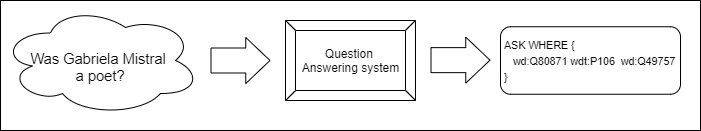
\includegraphics[scale=.5]{imagenes/1_intro/introQuestionAnsweringExample.png}
    \caption{Expected \SPARQL{} query example from a KGQA system.}
    \label{fig:introQAexample}
\end{figure}

The Query Template generator produces incomplete \SPARQL{} queries (which we call 
Query Templates) that contain \dquotesit{placeholders} in the position where entities are 
supposed to be (e.g. placeholders \texttt{<sbj\_1>} and \texttt{<obj\_1>} instead of entities 
\texttt{Q80871} and \texttt{Q49757} of the query shown in Figure~\ref{fig:introQAexample}). 
This module is built using the same model used to implement the baseline QAS. 
However, the training data is adapted to generate Query Templates instead of the complete 
query. This is achieved by removing the entities from the output \SPARQL{} queries included 
in the selected datasets such that the entities can rather be found by Entity Linking.

The role of the Entity Linking module is to recognize the relevant entities contained
in each question (e.g. identify that concepts \dquotesit{Gabriela Mistral} and \dquotesit{poet}
corresponds to the entities \texttt{Q80871} and \texttt{Q49757} in Figure~\ref{fig:introQAexample}) 
that are used to fill the Query Template. We implement various entity retrieval systems using 
one or more of the existing Entity 
Linking systems that have APIs available. The first variant is to use each EL system individually, 
which includes DBpedia Spotlight~\cite{EL:dbpedia-spotlight-MendesJGB11}, AIDA~\cite{EL:aida-tool-YosefHBSW11}, 
TAGME~\cite{EL:tagme-FerraginaS10}, and OpenTapioca~\cite{EL:opentapioca-Delpeuch19}. 
All of these systems, except for OpenTapioca, only work for DBpedia; therefore an 
extra mapping layer is implemented to map DBpedia entities to Wikidata entities. Two ensemble 
EL approaches are then proposed: one that prioritizes systems with higher Precision 
and another that implements a voting mechanism. We keep the variant that performs best 
according to the experiments that are explained in the \textit{Experimental results} subsection.

Additionally, a Slot Filling module is built by combining a Sequence Tagger model of the Flair 
library~\cite{seqlab:flair-AkbikBBRSV19} and a filling algorithm proposed in this work. Training 
the Sequence Tagger model requires building training data based on the selected datasets. 
Intuitively speaking, a Query Template may have multiple slots and multiple entities, where the 
Slot Filling module decides which entity should fill which slot (e.g. to infer that the concept 
\dquotesit{Gabriela Mistral} corresponds to the placeholder \texttt{<sbj\_1>}, therefore the 
entity \texttt{Q80871} should replace the occurrences of \texttt{<sbj\_1>} in the Query Template).

\subsection*{Experimental results}
\label{cap1:intro/contributions/expResults}
We conduct several experiments for validating each implemented module (Entity Linking, 
Slot Filling, and Query Template Generation) along with experiments over the defined 
benchmark for the end-to-end Question Answering process.

The Entity Linking systems are compared using Precision, Recall, and F1-score on the 
entities for each case on the dataset used for training. Testing is conducted over \QALDseven{} and 
our proposed dataset. The slot filling system is validated using Precision, Recall, and F1-score 
over the identified BIO labels (a common tagging format for sequence labeling tasks) over 
\LCQuADtwo{} and the mapped \DBNQA{} dataset. The query generator system is validated 
using BLEU score, Perplexity, and Accuracy over \LCQuADtwo{} and the mapped \DBNQA{} 
dataset. When training the query generator system, many split methods are tested according 
to the methodology proposed by Finegan-Dollak et al.~\cite{semPar:txt-to-sql-RadevKZZFRS18} for Text-to-SQL systems. 
The end-to-end Question Answering system is tested over all the datasets using the metrics 
described in the \textit{Benchmark on Question Answering over Wikidata} subsection.	
	%   Estructura del trabajo
	\section{Work Structure}
This worked is divided into the following chapters:

\begin{enumerate}
    \item In Chapter~\ref{cap2:theoFrame}, we describe the theoretical framework 
    enclosed on this work. This chapter covers concepts about what is the Semantic 
    Web, Information Extraction methods and how they relate with Semantic Web 
    technologies, Semantic Parsing applied on translating natural language to 
    \SPARQL, and the current state and challenges of the Question Answering over 
    Knowledge Graphs task.
    \item In Chapter~\ref{cap3:system}, we give an overview of the proposed Question 
    Answering system for this work. This includes a general explanation on the 
    pipeline proposed to generate a SPARQL query, and more specific details on how 
    each component is designed.    
    \item In Chapter~\ref{cap4:experimentalDesign}, we go into details about the 
    experiments we run on this work. We present the research questions we aimed to answer, 
    the baseline we compare our system with, and the metrics used to quantify the 
    performance of each system.    
    \item In Chapter~\ref{cap5:results}, we present the results derived from running the 
    proposed experiments. Aside from that, we include a brief discussion and analysis of 
    the results.    
    \item In Chapter~\ref{cap6:conclusions}, we summarize the conclusion of this work, 
    discuss its limitations and the future work regarding Question Answering over 
    Knowledge Graphs.
    
\end{enumerate}
	
\end{intro}
% Marco teorico
%   RDF y SPARQL
%   Entity Linking
%   Slot Filling
%   Redes Neuronales
%   Question Answering
\chapter{Theorical Framework}
	% Semantic Web
	\section{Semantic Web}
\label{cap2:semWeb}

\subsection{Web of Data}
\label{cap2:semWeb/webOfData}
During the short history of the World Wide Web, we have greatly benefited from how its 
content has been increasing every day while serving multiple purposes. This vast amount of 
knowledge has become humanly impossible to traverse, so we rely on machines to 
process the content of documents automatically. As Hogan mentions, machines require the 
data to fulfill two primary requirements in order to be able to process them automatically 
in a meaningful way: to have a machine-readable structure and semantics~\cite{key:linked14-Hogan}. 
Unless a more \dquotes{formal} notion of structure and semantics is provided, machines can not 
be used to their full potential.

Various standards have emerged to partially structure the Web’s content, such as XML, CSV, 
or JSON. However, structured content without some semantics does not permit machines to do 
much more than split the content up by its delimiters and load its structure. Some other 
standards define semantic meaning for their structure, where some prominent examples are 
HTML, RSS or XML Schema (XSD), but often the semantics are defined in a human-readable way, 
for example, to describe how certain HTML elements should be rendered in a browser. Though 
these markup-based specifications provide a set of terms that often serve a singular purpose 
within the context of a given application, their interpretation tends to differ significantly 
for the respective consumer applications. 

The multiple purposes that standards like HTML can serve are not able to address some of the 
shortcomings of the current Web. Since content is often created to serve specific functionalities 
in the context of a given site, much of this content ends up not being directly reusable, 
high levels of redundancy appear or it cannot be integrated with other sites. In an effort 
to address these limitations, the Semantic Web was proposed.

The Semantic Web is designed as an extension of the current World Wide Web so as to enable 
the creation, sharing, and intelligent re-use of machine-readable content on the Web. The 
inception of the modern notion of the Semantic Web is founded on two major milestones: the 
original W3C recommendation of the first Resource Description Framework (\RDF{}) standard 
defining the core data model~\cite{key:oldrdf}, and the introduction of the vision for the 
Semantic Web outlined by Berners-Lee et al.~\cite{key:semwebsa}.

The vision of the Semantic Web can be represented through the Semantic Web Stack, first 
conceived by Berners-Lee et al., as seen in Figure~\ref{fig:semanticWebStack}. The lower levels describe the 
foundational elements of the Semantic Web which are aligned with the Web itself. First, 
the Web needs some standard to map from binary-streams and storage to textual information, 
so it relies on \textbf{Characters} from the standard Unicode character-set. Then, \textbf{Identifiers} 
respond to the main purposes of denoting any concept or concrete thing. The natural choice is to 
use Uniform Resource Identifiers (URI), which is the native standard for identification on 
the Web, or a recently adopted generalization of URI, Internationalized Resource 
Identifiers (IRI), which additionally support unescaped Unicode strings. The \textbf{Syntax} layer 
serves the objective of allowing machines to automatically parse content into its elementary 
components by defining syntaxes with formally defined grammars. For example, one of the most 
common syntaxes used to encode Semantic Web data is the Terse RDF Triple Language (Turtle) 
syntax~\cite{key:turtle}, based on the Notation3 (N3) syntax~\cite{key:n3}.

\begin{figure}[!h]
    \centering
    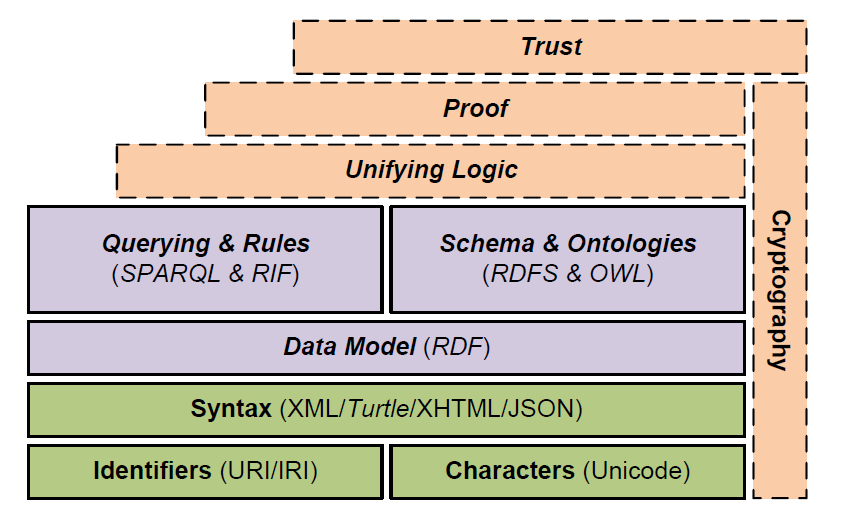
\includegraphics[scale=.65]{imagenes/2_theorical_framework/semanticWebStack.png}
    \caption{Semantic Web Stack~\cite{key:linked14-Hogan}}
    \label{fig:semanticWebStack}
\end{figure}

The next set of layers forms the core of the Semantic Web. The \textbf{Data Model} layer 
provides a canonical representation where machines can exchange machine-readable data in 
a generic framework. The core data-model for the Semantic Web is the Resource Description 
Framework (\RDF{})~\cite{key:rdfprimer}. In order to bring some meaning to the \RDF{} content, 
it requires formal languages whose meta-vocabulary complement the \RDF{} data-model by providing 
well-defined semantics. These languages correspond to the \textbf{Schema \& Ontologies} layer, 
where the RDF Schema (RDFS)~\cite{key:oldrdf} and Web Ontology Language (OWL)~\cite{key:owloverview, key:owl2rationale} 
standards are the essential languages integrated as part of the current Semantic Web. 
Eventually, the content described in \RDF{} needs to be processed by declarative querying 
and rules languages that serve many purposes, like generating results for user interfaces 
or inferring novel \RDF{} data. The \textbf{Querying \& Rules} layer is where the querying 
and rules standards for the Semantic Web are defined. In this case, the \textit{SPARQL Protocol 
and RDF Query Language}~\cite{key:sparql,key:sparql11protocol,key:sparql11} 
defines the querying standards and the Rule Interchange Format (RIF)~\cite{key:rifframework} 
defines the rules standards.

The top and side of the stack in Figure~\ref{fig:semanticWebStack} are layers yet to be realized. Though many 
proposals have been made in the research literature, no mature standards or tooling have 
emerged. The remaining top layers aim to combine the described low-level technologies into 
a unifying language to execute queries and rules over knowledge represented in \RDF{} 
(Unifying Logic), provide proofs to validate procedures or information used (Proof), and 
determine the trustworthiness of information sources (Trust). The Cryptography side layer 
is centered on cryptographic techniques for verifying and allowing access control mechanisms.

Providing more details on this broad overview of the Semantic Web, we start by focusing on 
how data is represented and how querying the content is described by any selected source. 
Then, in the following sections, we go deeper into understanding the Semantic Web data-model, 
\RDF{}, and its querying standard, \SPARQL{}.

\subsection{Resource Description Framework}
\label{cap2:semWeb/rdf}
The \textbf{Resource Description Framework} (\RDF{}) standard~\cite{key:rdfprimer} provides 
a data-model on the Semantic Web, which can be serialized using the Turtle syntax~\cite{key:turtle}. 
Having this data-model allows for any content framed in \RDF{} to be generically processed 
and indexed by external systems, whatever its topic or origin. The atomic elements that 
constitute the \RDF{} data-model are called \textbf{\RDF{} Terms}. \RDF{} does not follow the Unique 
Name Assumption (UNA), so two \RDF{} terms can refer to the same referent. The set of \RDF{} terms 
are divided into three disjoint subsets: URIs, Literals and Blank Nodes.

As mentioned previously, \textbf{Uniform Resource Identifiers} serve as identification for 
any resource. An example to identify the country Chile in DBpedia~\cite{KG:dbpedia} is 
the URI \url{http://dbpedia.org/resource/Chile}. A shorter version can be used 
by using the CURIE-style shortcuts~\cite{key:prefixes}, where a re-usable prefix can be 
defined: \texttt{@prefix dbr: <\url{http://dbpedia.org/resource/}>}. This way, the 
identifier of Chile can be abbreviated to \texttt{dbr:Chile}.

% note: ^ is \textasciicircum, ~ is \textasciicircum, \ is \textbackslash
\textbf{Literal} values represent lexical values and are divided into two categories. 
Plain literals are a set of plain strings, such as \texttt{\dquotes{Hello World}}, and can 
include an associated language tag, such as \texttt{\dquotes{Hello World}@en}. Typed 
literals are literals that include a datatype, such as 
\texttt{\dquotes{8}\textasciicircum\textasciicircum xsd:int}. Datatypes are identified by 
URIs (such as \texttt{xsd:int}) and borrow most of the datatypes defined for XML 
Schema~\cite{key:xsd}. Datatypes are often used for data validation or mapping.

\textbf{Blank Nodes} are used as existential variables that denote the existence of some 
resource without having to explicitly reference it using a URI or literal. The scope of a 
blank node is limited to the local \RDF{} document where it is defined, so it cannot be 
referenced elsewhere. In Turtle, blank nodes can be referenced explicitly with an 
underscore prefix \texttt{\_:bnode1} or implicitly in a variety of other manners.

\RDF{} terms are then combined together to form \RDF{} Triples. As its name suggests, a triple 
is a 3-tuple of \RDF{} terms. The three components of a triple are commonly called subject, 
predicate and object. \RDF{} triples can be seen as an atomic representation of a 
\dquotes{fact} or \dquotes{claim}, e.g. \dquotesit{Santiago is the capital city of Chile}. 
Typically each \RDF{} triple position fulfills a certain role: the subject is the primary 
resource that is being described (either a URI or a blank node), the predicate is the 
relation between the subject and the object (must be a URI), and the object is the value 
of the relation (any of the mentioned \RDF{} terms). For instance, we illustrate the Turtle 
representation of a set of \RDF{} triples from DBpedia in Listing~\ref{lst:dbpediaRdfExample}.

\begin{sparqlcode}[caption={Set of \RDF{} triples about Gabriela Mistral in DBpedia using Turtle syntax.},label={lst:dbpediaRdfExample}]
# PREFIX DECLARATIONS
@prefix dbr: <http://dbpedia.org/resource/>
@prefix dbo: <http://dbpedia.org/resource/>
@prefix dbp: <http://dbpedia.org/resource/>
@prefix rdfs: <http://www.w3.org/2000/01/rdf-schema#>

# RDF TRIPLES
dbr:Gabriela_Mistral rdfs:label "Gabriela Mistral"@en .
dbr:Gabriela_Mistral dbp:occupation dbr:Poet .
dbr:Gabriela_Mistral dbo:birthPlace dbr:Vicuña,_Chile .
dbr:Gabriela_Mistral dbo:awards dbr:Nobel_Prize_in_Literature .
dbr:Gabriela_Mistral dbo:awards dbr:National_Prize_for_Literature_(Chile) .
dbr:Vicuña,_Chile rdfs:label "Vicuna, Chile"@en .
dbr:Vicuña,_Chile dbo:populationTotal 25085 .
dbr:Vicuña,_Chile dbo:isPartOf dbr:Elqui_Province .
dbr:Vicuña,_Chile dbo:isPartOf dbr:Coquimbo .
dbr:Vicuña,_Chile dbo:country dbr:Chile .
\end{sparqlcode}

Listing~\ref{lst:dbpediaRdfExample} shows facts about Gabriela Mistral, a famous Chilean poet, 
and how those facts are structured as a set of \RDF{} triples, where each triple is separated by a 
dot symbol. The use of CURIE-style prefixes helps to simplify the content and make it easier to 
understand for a human reader~\cite{key:prefixes}. Moreover, Listing~\ref{lst:dbpediaShortRdf} 
shows how Turtle allows for abbreviating the content by grouping triples with common subjects 
(using the \squotestt{;} symbol) or predicates (using the \squotestt{,} symbol).

\begin{sparqlcode}[label={lst:dbpediaShortRdf},caption={Set of \RDF{} abbreviated triples about Gabriela Mistral in DBpedia.}]
...
# RDF TRIPLES
dbr:Gabriela_Mistral rdfs:label "Gabriela Mistral"@en ;
    dbp:occupation dbr:Poet ;
    dbo:birthPlace dbr:Vicuña,_Chile ;
    dbo:awards dbr:Nobel_Prize_in_Literature, dbr:National_Prize_for_Literature_(Chile) .
dbr:Vicuña,_Chile rdfs:label "Vicuña, Chile"@en ;
    dbo:populationTotal 25085 ;
    dbo:isPartOf dbr:Elqui_Province , dbr:Coquimbo ;
    dbo:country dbr:Chile .
\end{sparqlcode}

Given the triple-based structure of \RDF{} triples, it is possible to represent entire 
datasets as an \RDF{} graph, also known as a \textbf{Knowledge Graph} (KG): a directed labeled 
graph where subjects and objects are represented by nodes, and predicates are represented 
by the directed edges that bond two nodes. The \RDF{} graph of the example shown above can be 
drawn as in the diagram of Figure~\ref{fig:dbpediaGraphExample}, where by convention 
ellipses correspond to URIs or blank nodes, and rectangles symbolize literals.

\begin{figure}[!h]
    \centering
    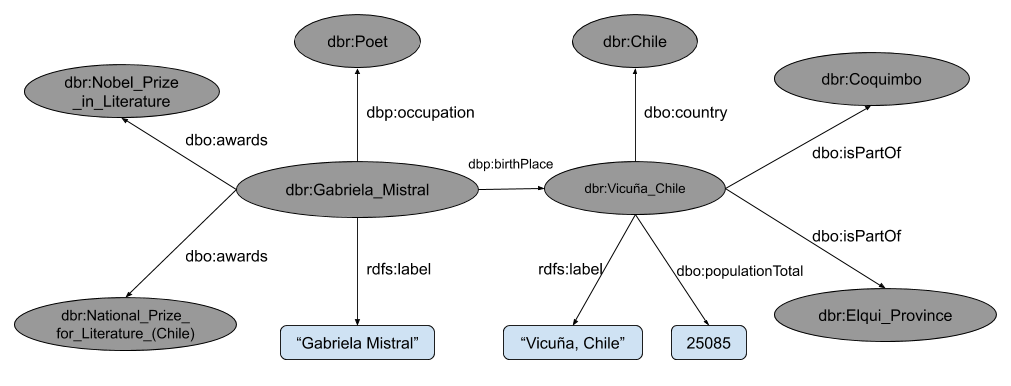
\includegraphics[scale=.55]{imagenes/2_theorical_framework/exampleDbpediaGraph.png}
    \caption{\RDF{} graph representing facts about Gabriela Mistral from Listing~\ref{lst:dbpediaRdfExample}.}
    \label{fig:dbpediaGraphExample}
\end{figure}

Besides \RDF{} triples and \RDF{} graphs, \RDF{} standards provide a rich set of built-in 
vocabulary terms under a core \RDF{} namespace, which helps to standardize frequently used 
\RDF{} patterns. One popular term is \texttt{rdf:type}, which helps to assign resources 
sharing certain commonalities into \textbf{classes}. For example, we can denote 
\texttt{dbr:Vicuna\_Chile} as a city by combining it with the predicate \texttt{rdf:type} 
and the object \texttt{dbr:City}. Another example is the term \texttt{rdfs:label} that 
comes from RDF Schema~\cite{key:rdfsold}, which provides other resources for describing 
relations such as \textbf{subproperties} or \textbf{subclasses}. Though our work is not 
focused on the use of the Web Ontology Language (OWL)~\cite{key:owl2rationale, key:owloverview}, 
it is worth mentioning that it also adds a wealth of new vocabulary to describe new 
relations between resources like equivalences, disjointness, inverse properties, among others.

Ultimately, there are numerous syntaxes for writing \RDF{} apart from Turtle~\cite{key:turtle}, among 
which we can name RDF/XML~\cite{key:rdfxml}, N-Triples~\cite{key:testcases}, RDFa~\cite{key:rdfa11p, key:rdfa}, 
and JSON LD~\cite{key:jsonld}. However, no matter what syntax is chosen, every one is 
represented in the same \RDF{} data model; thus it is possible to convert any \RDF{} content 
in one syntax to another while keeping the same \RDF{} data.

\subsection{SPARQL Query Language}
\label{cap2:semWeb/sparql}
The \textbf{SPARQL} protocol defines how \SPARQL{} queries retrieve results over the \RDF{} 
data-model~\cite{key:sparql11protocol}. These standards became W3C Recommendations in 
2008~\cite{key:sparql} and then were extended in 2013 in the SPARQL 1.1 version~\cite{key:sparql11} 
superseding the previous W3C Recommendations. Some \SPARQL{} query features and keywords are similar 
to the ones found in the Structured Query Language (SQL), though \SPARQL{} is designed for interacting 
with \RDF{} data.

\begin{sparqlcode}[%
    caption={\SPARQL{} query for getting awards won by people who were born in Vicuña.},
    label={lst:dbpediaSparqlExample}]
# PREFIX DECLARATIONS
PREFIX dbr: <http://dbpedia.org/resource/>
PREFIX dbo: <http://dbpedia.org/ontology/>
# DATASET CLAUSE
FROM <http://dbepdia.org/data/Gabriela_Mistral.ttl>
# RESULT CLAUSE
SELECT ?people ?award
# QUERY CLAUSE
WHERE {
    ?people dbo:birthPlace dbr:Vicuña,_Chile ;
        dbo:award ?award .
}
# SOLUTION MODIFIERS
LIMIT 2
\end{sparqlcode}

There are five main components that describe a \SPARQL{} query. First, \textbf{Prefix Declarations} 
serve as shortcuts for later in the query, similar to the Turtle shortcuts. Following prefixes, 
the \textbf{Dataset Clause} allows for specifying one or more \RDF{} graphs over which the query 
should be executed. When no dataset clause is specified, query patterns are matched against the 
default graph which usually corresponds to all of the data loaded and indexed. The 
\textbf{Result Clause} indicates what type of query is being executed and what results are expected. 
The most relevant part is the \textbf{Query Clause}, where the query patterns to match against the 
data are specified and used to generate variable bindings. Finally, the \textbf{Solution Modifiers} 
permit to order, slice or paginate the results. Note that the only mandatory part is the result 
clause, though most queries also include at least one query clause. An example of a \SPARQL{} query is 
represented in Listing~\ref{lst:dbpediaSparqlExample}, where we are looking for which awards 
people who were born in Vicuña have won.

For example, if the \RDF{} triples shown in Listing~\ref{lst:dbpediaRdfExample} were contained in the 
\RDF{} graph \texttt{<\url{http://dbpedia.org/data/Gabriela\_Mistral.ttl}>}, the results 
expected from the \SPARQL{} query in Listing~\ref{lst:dbpediaSparqlExample} would be as shown 
in Table~\ref{table:dbpediaExampleResults}.

\begin{table}[h!]
    \centering
    \begin{tabular}{ |c|c| }        
        \hline
        ?people & ?award \\ 
        \hline
        dbr:Gabriela\_Mistral & dbr:Nobel\_Prize\_in\_Literature \\
        dbr:Gabriela\_Mistral & dbr:National\_Prize\_for\_Literature\_(Chile) \\
        \hline
    \end{tabular}
    \caption{Results from \SPARQL{} query example in Listing~\ref{lst:dbpediaSparqlExample}.}
    \label{table:dbpediaExampleResults}
\end{table}

There are four types of \SPARQL{} queries, which are defined by the first keyword used in the 
\textit{Result Clause}. The example shown above is a \texttt{SELECT} query, which requests a list 
of bindings for variables specified in the \textit{Query Clause}. Since a \texttt{SELECT} query 
returns duplicate results by default, it can include either the \texttt{DISTINCT} keyword to filter 
duplicate results, or the \texttt{REDUCED} keyword that may allow duplicates such that the engine 
can choose whatever it deems to be more efficient. An \texttt{ASK} query returns a boolean value 
indicating whether or not the query’s results are non-empty. A \texttt{CONSTRUCT} query provides 
an \RDF{} template with placeholders to be filled later, thus returning an \RDF{} graph according to 
those inserted variables. The last type is the \texttt{DESCRIBE} query, which provides an \RDF{} 
description for a particular \RDF{} term. For this work we only focus on \texttt{SELECT} and 
\texttt{ASK} type queries.

Knowing how to define the content inside a \textit{Query Clause} is crucial in order to specify what results 
a \SPARQL{} query should return. There are many core features defined over the basic graph patterns 
that are used to create complex query patterns in query clauses. Among these patterns, we highlight 
the \texttt{FILTER} keyword that serves to establish conditions that a query solution should match. 
These conditions can be constructed from a broad arsenal of tools: arithmetic operators and 
comparators, built-in functions, casting, boolean connectives and even user-defined functions. 
We also mention the \texttt{UNION} operator, that allows joining results from two groups of query 
patterns. Another important feature is the \texttt{OPTIONAL} feature, which allows for matching 
data if available (if not, the corresponding result is still returned, where the variables 
exclusive to the \texttt{OPTIONAL} clause are left unbound).

After retrieving results from the \textit{Query Clause}, such results can be divided or modified. 
The \texttt{ORDER BY} operation sorts results in ascending (\texttt{ASC}) or descending (\texttt{DESC}) order based 
on one or more variables; and the \texttt{LIMIT} keyword restricts the amount of results to return. 
Finally, the \texttt{OFFSET} clause allows the query to skip a certain number of results.

Besides the basic operations provided by the original \SPARQL{} standard, the later update to 
SPARQL 1.1~\cite{key:sparql11} brought a wide-range of new features that increase the expressiveness 
and capabilities of this query language. Some core additions are property paths, aggregation, 
binding variables, subqueries, updates, new format outputs (CSV, TSV, JSON), among others. 
For this work we want to highlight the use of \textit{property paths} and \textit{aggregation} 
that will be often used. \textit{Property paths} allow the user to match paths of arbitrary 
length in an \RDF{} graph using regular expressions. \textit{Aggregation} techniques include 
operations like count, max, min, sum, etc.; and can be applied over query results grouped 
by common terms.

Though many other \SPARQL{} features are left to be mentioned, we focused on the features described 
above since those are the important ones for the development of this work.

\subsection{Linked Open Data Cloud}
\label{cap2:semWeb/linkedData}
Having briefly mentioned some core components of the Semantic Web, we have scratched just a tiny 
portion of what the Semantic Web concept means, and how it can be deployed on the Web. Most of 
what defines the use of the Semantic Web on the Web itself resides in understanding 
\textbf{Linked Data}. The early attempts to publish \RDF{} on the Web tended to produce large dumps 
of data rarely interlinked with other \RDF{} datasets and using different conventions. These issues 
ended up leaving entire isolated islands of \RDF{} datasets that were difficult to access and with 
little chance of being discovered by other communities. Therefore, \textit{Linked Data} emerged as 
a set of principles and best practices~\cite{key:ldprinciples} to provide an environment where 
Semantic Web standards can be effectively deployed on the Web.

The four Linked Data principles arise from the Web Design Issues document published by 
Berners-Lee~\cite{key:ldprinciples}. According to this document, these principles are: (1) use URIs 
as names for things, (2) use HTTP URIs so those names can be looked up, (3) return useful 
information upon lookup of those names, and last (4) include links by using URIs that dereference 
to remote documents. 

Besides these principles, there is an emphasis on publishing data that can be easily processed, 
reused and exchanged between machines. As an approach to bootstrap Semantic Web publishing, 
a 5-star system~\cite{key:ldprinciples} was promoted to describe the quality of published \RDF{} data. 
Each star corresponds to one of the following considerations: (1) publish data under an open license, 
(2) publish structured data, (3) use non-proprietary formats, (4) use URIs to identify things, and 
(5) link the published data to other data.

A community project named \dquotesit{Linking Open Data}, supported by W3C and inspired by the growth 
in Open Data, emerged to promote these Linked Data principles~\cite{key:ldbook}. The community 
project aims to introduce the benefits of Semantic Web technologies to the Open Data movement and 
to bootstrap the Web of Data by including many emerging open datasets. The community published 
guidelines are based on the core principles mentioned before. Among those guidelines, the main 
ones are:

\begin{itemize}
    \item \textbf{Dereferencing practices}: describes how to identify and perform lookups 
    for either entities or documents. This includes recommendations on indirect URIs to signify 
    distinctions on a HTTP level or providing as detailed an \RDF{} description as possible when 
    dereferencing resources. 
    \item \textbf{Linking Aliases}: allow the use of multiple URI aliases that refer to the same 
    thing. For example, \texttt{owl:sameAs} links can be used to specify equivalence between 
    resources in different datasets.
    \item \textbf{Describing Vocabularies Terms}: promotes the shared use of common vocabularies 
    of class and property terms. A common example is to use FOAF to describe people.
    \item \textbf{Provision of SPARQL Endpoints}: though not required, providing a \SPARQL{} endpoint 
    for a given Linked Data site gives consumers a single-point-of-access to query over the merge 
    of contributions on that site.
\end{itemize} % TODO: check why itemize put so much space between items (removing following section line reduces the space to normal)

Based on these standards and guidelines, the \textbf{Linking Open Data Cloud}, a set of more than 
300 different interlinked \RDF{} datasets, has been constantly growing and including a wider range of 
topics. Some of the most relevant datasets are DBpedia~\cite{KG:dbpedia}, whose content is mostly 
based on Wikipedia articles, Freebase~\cite{KG:freebase}, a dataset previously supported by Google, 
and Wikidata~\cite{KG:wikidata}, a large dataset supported by its community. Our work is mainly 
focused on the latter knowledge graph, which we will introduce in the next section.

\subsection{Wikidata}
\label{cap2:semWeb/wikidata}
As described by Vrandečić and Krötzsch~\cite{KG:wikidata}, \textbf{Wikidata} is a free 
collaborative Knowledge Graph founded by the Wikimedia Foundation\footnote{\url{https://wikimediafoundation.org/our-work/wikimedia-projects/}} 
in October 2012. Given the constant growth of its sister project Wikipedia, one of the most 
popular online encyclopedias, Wikidata is introduced as a new multilingual 
\dquotesit{Wikipedia for data}. 

Despite Wikipedia’s rich amount of data, consisting of more than 30 million articles in at least 
287 languages, it started to face serious limitations in terms of providing data easily to the 
community~\cite{KG:wikidata}. There was the lack of direct access through query services or 
downloadable data exports, the same information often needed to be manually maintained in the 
same articles across many languages and across many articles within a single language, among 
others limitations. Wikidata aims to overcome many of Wikipedia’s limitations by managing its 
data centrally.

Wikidata offers many features that make it an attractive and potentially useful resource for 
sharing information and connecting communities. Some aspects to consider about Wikidata are:

\begin{itemize}
    \item \textbf{Openly editable}: allows any user to extend and edit the stored information.
    \item \textbf{Community control}: contributor community control that not only supervises the 
    data being published but also the schema of the data. 
    \item \textbf{Plurality}: though many facts can be disputed or be uncertain, Wikidata provides 
    mechanisms to organize conflicting data for coexisting together.
    \item \textbf{Secondary data}: gathers facts published in primary sources including references 
    to these sources.
    \item \textbf{Multilingual data}: all data have universal meaning and most of it is not tied 
    to a single language. There is only one universal version of Wikidata.
    \item \textbf{Easy access}: data published under liberal legal terms are made  easily 
    accessible through web services, allowing the widest possible reuse.
    \item \textbf{Continuous evolution}: Wikidata grows with its community of editors and 
    developers, so new features are constantly being added.
\end{itemize}

Wikidata has its own data model but further offers exports that follow the Semantic Web 
standards~\cite{key:wikidataErxlebenGKMV14}. To identify items, Wikidata provides unique IDs, 
which are highly reusable and provide unambiguous definitions that do not depend on language 
labels. The same example of the entity Chile mentioned before is now represented in Wikidata as 
\texttt{\url{http://www.wikidata.org/wiki/Q298}}. 

\begin{sparqlcode}[%
    caption=Set of RDF triples about Gabriela Mistral in Wikidata., 
    label=lst:wikidataRdfExample]
# PREFIX DECLARATIONS
@prefix wd: <http://wikidata.org/wiki/>
@prefix wdt: <http://wikidata.org/prop/direct/>
@prefix p: <http://wikidata.org/prop/>
@prefix pq: <http://wikidata.org/prop/qualifier/>
@prefix rdfs: <http://www.w3.org/2000/01/rdf-schema#>

# RDF TRIPLES
# Gabriela Mistral
wd:Q80871 rdfs:label "Gabriela Mistral"@en ;
    wdt:P106 wd:Q49757 ;
    wdt:P19 wd:Q201007 ;
    wdt:P166 wd:Q37922, wd:Q860699 .
# Vicuna
wd:Q201007 rdfs:label "Vicuña"@en ;
    p:P1082 _:population2017 ;
    wdt:P131 wd:Q721224 ;
    wdt:P17 dbr:Chile .
_:population2017 pq:P1082 25085
# Elqui Province
wd:Q721224 wdt:P131 wd:Q2121 .
\end{sparqlcode}

Since some facts cannot be directly expressed by simply using the property-value convention, 
like the population of Chile across different years, Wikidata also provides additional 
subordinate property-value pairs called \dquotesit{qualifiers}. \textbf{Qualifiers} can be used 
to state contextual information such as validity time or ternary relations (e.g. cast members of 
a movie with their role). Another way to understand qualifiers is by looking at Wikipedia 
infoboxes which have a similar data representation.

\begin{figure}[!h]
    \centering
    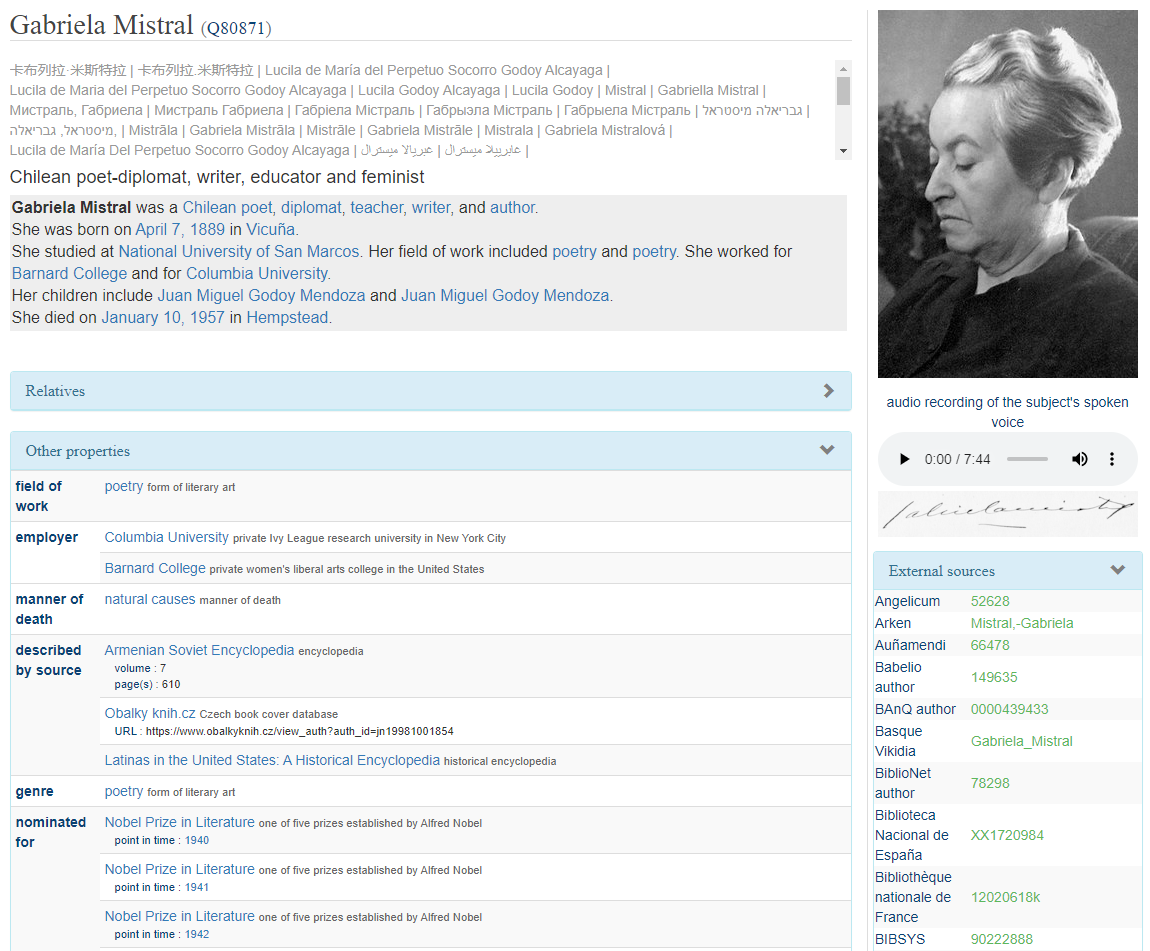
\includegraphics[scale=.5]{imagenes/2_theorical_framework/wikidataReasonatorExample.PNG}
    \caption[Example of an external application of Wikidata using Reasonator.]{Example of an external application of Wikidata using Reasonator\footnotemark.}
    \label{fig:wikidataReasonator}
\end{figure}

\footnotetext{\url{https://reasonator.toolforge.org/?&q=80871}}

For a better understanding, let us recall the same data about Gabriela Mistral, but now using 
Wikidata resources, as shown in Listing~\ref{lst:wikidataRdfExample}. Since different knowledge 
graphs do not necessarily represent the same information in the same way, we can appreciate slight 
differences like how the city Vicuña is described. In this case, Vicuña is not directly represented 
as part of Coquimbo but instead only the Elqui Province. Nevertheless, both representations are 
intrinsically correct since both are portraying the same fact. Another difference is the use of 
a Wikidata property qualifier to denote that the population for Vicuña shown in 
Listing~\ref{lst:wikidataRdfExample} is the population of 2017, in contrast to the DBpedia 
representation, shown in Listing~\ref{lst:dbpediaShortRdf}, which does not show that fact.

Ultimately, the data in Wikidata lends itself to numerous applications on very different levels 
of data integration. Wikidata provides many language labels and descriptions for many terms in 
different languages, which allows any service to present and/or or translate information for 
various audiences. Some applications are built to access Wikidata’s data more conveniently and 
effectively. One example is illustrated by Figure~\ref{fig:wikidataReasonator}, showing 
information about Gabriela Mistral retrieved by the data browser 
\textit{Reasonator} using the Wikidata API. Additionally 
applications can be enriched with information provided by Wikidata, such as how Google Maps 
uses Wikidata’s geographical labels to enhance its application interface. 

On a more advanced level, many research analyses can be performed over the information in 
Wikidata in order to derive new insights beyond its surface data. A couple of potential examples 
are analyses using logical reasoning to understand intrinsic meaningful relationships among 
entities, or statistical evaluations over the data to analyze biases like the ones that involve 
language coverage~\cite{key:wikidataHale13} or gender balance~\cite{key:socialWikidataWagner16}. 
Wikidata is already an important platform and has the potential to be a major resource for both 
researchers and developers~\cite{wikidata:GeneWikiInitiative, wikidata:RiseWikidataVrandecic6682924}.
	
	% Information Extraction
	\section{Information Extraction}
\label{cap2:theoFrame/infExtr}
\subsection{Information Extraction methods with Semantic Web technologies}
\label{cap2:theoFrame/infExtr/methods}
As the Semantic Web aims to make structured data available enabling high levels of 
automation, there are still some challenges regarding the increasing demand for information. 
There is still a gap between the coverage of structured and unstructured data on the 
Web~\cite{infExtr:PolleresHHD10}. However, making high-quality annotations on unstructured 
data is not a trivial task because it requires processing vast amounts of information that 
is constantly changing. 

Thus, automatic techniques for extracting and annotating information have gotten more 
attention in the context of the Semantic Web. As described by Martinez et. al., Information 
Extraction (IE) refers to the automatic extraction of implicit information from unstructured 
or semi-structured sources~\cite{infExtr:MartinezHL19}. IE methods are used to identify 
entities, concepts and/or semantic relations implicit in an input source, typically a text 
in natural language. 

Many systems have been developed to automate the extraction or enrichment of Semantic Web 
resources such as ontologies, knowledge graphs, etc. These systems are often based on 
Information Extraction methods which usually rely on techniques from areas such as Natural 
Language Processing, Machine Learning and Information Retrieval. 

The combination of tools from the Semantic Web and Information Extraction areas presents two 
perspectives: using Information Extraction to populate the Semantic Web, or using Semantic 
Web resources to improve Information Extraction processes. In this work we focus on the last 
perspective mentioned, in particular how to extract and link entities over unstructured input 
sources (such as natural language questions).

An entity is understood as an atomic element within a Semantic Web knowledge base or ontology. 
Entity Extraction \& Linking (EEL) is then the task of identifying mentions in a text or 
document, and linking them as entities to one or more reference knowledge graphs. EEL is 
typically divided into two main steps: a recognition stage where relevant named entities are 
identified, and a disambiguation stage, where entities are mapped to candidate resources in 
the knowledge graph and subsequently ranked. Entity extraction often uses off-the-shelf Named 
Entity Recognition (NER) tools to recognise relevant entities. After extraction, Entity 
Linking follows, where the disambiguation of the spotted mentions links each mention to an 
identifier in a target knowledge graph, and may include a score or weight calculation that 
denotes the confidence or support over the output annotations. We now discuss the Entity 
Linking process in more detail.

\subsection{Entity Linking}
\label{cap2:theoFrame/infExtr/entityLinking}
Entity Linking is the task of linking mentions in text to their corresponding entities in a 
knowledge graph (e.g. Wikipedia, Wikidata, DBpedia)~\cite{EL:survey-WuHH18}. Aside from 
extracting entities from a knowledge graph, a disambiguation step is also needed. For example, 
for the question \textit{“Has Claudio Bravo played for Manchester City FC?”}, Entity Linking 
with respect to Wikidata should link the mention \textit{“Claudio Bravo”} to the Chilean 
football goalkeeper Claudio Bravo (wd:Q313161) instead of the Chilean painter Claudio Bravo 
(wd:Q491787), given the context of the sentence (a person playing in a football club). Some 
applications of Entity Linking involve fields such as information 
retrieval~\cite{infExtr:CornoltiFCRS16, infExtr:BlancoOM15, infExtr:BollegalaMI07} knowledge 
fusion~\cite{infExtr:DongGHHMSZ15, infExtr:BohmFHLMNEHHS12}, or knowledge base 
population~\cite{infExtr:RaoMD13, infExtr:DredzeMRGF10, infExtr:FreedmanMM17}.

Commonly, the entity linking process is divided into three modules: candidate entity 
generation, candidate entity disambiguation and linking the result. A formal description of 
Entity Linking according to Wu and He~\cite{EL:survey-WuHH18} is the following: Given a set of 
documents $d=\{d_1,d_2,\ldots\}$ and a knowledge base $K$, we can get a mention set 
$M=\{m_1, m_2,\ldots\}$ using a Named Entity Recognition tool. For each $m_i \in M$, we can 
get a candidate set $C=\{c_1, c_2,\ldots\}$ from a knowledge base. The goal of Entity Linking 
is to choose an entity from $c \in C$ for each mention $m \in M$. If $score(m,c)$ is below 
$\tau$ ($\tau$ is a threshold) for all $c \in C$, then the target entity of m is 
\textit{Not In Lexicon} (NIL); otherwise, $m$ will be linked to $c'$ such that 
$score(m,c')=max\{score(m,c) \mid c\in C \}$. Figure~\ref{fig:entitylinkingGeneralModel} shows a 
general model including each phase and the formal description mentioned.

\begin{figure}[!h]
    \centering
    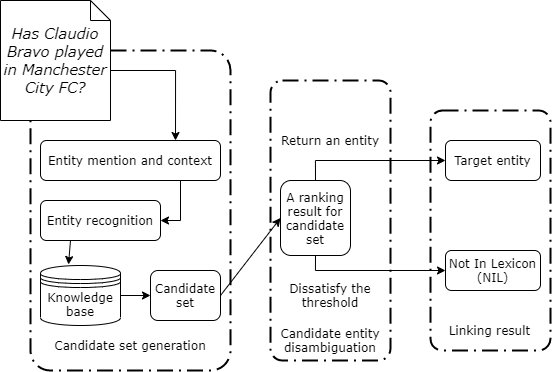
\includegraphics[scale=.5]{imagenes/2_theorical_framework/information_extraction/entityLinkingModel.PNG}
    \caption{A general model of Entity Linking based on Wu and He~\cite{EL:survey-WuHH18}}
    \label{fig:entitylinkingGeneralModel}
\end{figure}

The first module selects the candidate entities for each mention identified in the text and 
finds related entities in the knowledge base. For example, \textit{Claudio Bravo} is related 
to the entities \textit{Claudio Bravo (football goalkeeper)} and \textit{Claudio Bravo (painter)}.

The second module ranks the candidate entities by combining different features of 
entities and assigning scores to each candidate. Some features could be entity popularity, 
entity type, similarity between names or context in the query, topic similarity and a 
combination of several features. In the example, \textit{Claudio Bravo (football goalkeeper)} 
should have a higher score than \textit{Claudio Bravo (painter)} due to the football-related 
context of the sentence. 

The last module selects the target entity for each mention according to the ranking derived 
from the previous module. The candidates with the highest score per mention are selected 
among the candidates whose scores are above the threshold. If scores from all candidates are 
below the threshold, some systems return a NIL clustering~\cite{infExtr:ji2010overview}, 
although we will work with systems that directly discard results that do not satisfy the 
threshold.

There are various existing methods for addressing candidate entity generation and 
disambiguation. The methods for candidate entity generation can be divided into methods 
based on dictionaries~\cite{infExtr:ZhangSTW10, infExtr:HanSZ11}, 
direct search~\cite{infExtr:McNameeMLOD11, infExtr:DredzeMRGF10} and 
probabilistic methods~\cite{infExtr:ganea2016, infExtr:PanCHJK15}. On the other hand, the 
methods for candidate entity disambiguation can be divided into methods based on 
similarity computation~\cite{infExtr:Cucerzan07, infExtr:BunescuP06}, 
machine learning~\cite{infExtr:ganea2016, infExtr:ZhangSTW10} 
and graphs~\cite{infExtr:GongFLSH17, infExtr:HanSZ11}.

One of the main difficulties in Entity Linking is the high ambiguity of entity mentions, 
which make it more difficult to understand the meaning of entity mentions. These ambiguities 
include polysemies, which refer to mentions that correspond to many entities (e.g. 
\textit{Claudio Bravo}) or multiword synonyms, which refer to entities that may have many 
kinds of surface forms (e.g. \textit{Manchester City FC} is also known as \textit{The Citizen} 
or \textit{The Sky Blues}). Another problem happens when selecting entities in the linking 
results phase since the threshold is selected manually and can lead to the problem that 
correct targets can be below the threshold, thus being discarded.

Entity linking evaluation criteria are usually based on Precision, Recall and 
F1-score. For each of these metrics there is a micro measure and a macro 
measure~\cite{entlin:CornoltiFC13}. The macro measure gives equal importance to each 
document since it first calculates the relevant measure over each document, and then 
calculates the arithmetic average. On the other hand, the micro measure considers all 
mentions as part of one document when calculating the relevant measure, thus giving more 
importance to documents with more mentions. The following equations represent the micro and 
macro measures of Precision and Recall:
% E --> G, G --> S
\begin{align*} 
    Precision_{micro} = \frac{|S \cap G|}{|S|} \\
    Recall_{micro} = \frac{|S \cap G|}{|G|} \\
    Precision_{macro} = \frac{\sum_{i=1}^{|D|} \frac{|s_i \cap g_i |}{|s_i|}}{|D|} \\
    Recall_{macro} = \frac{\sum_{i=1}^{|D|} \frac{|s_i \cap g_i |}{|g_i|}}{|D|}
\end{align*}
\noindent where $D$ represents a document containing a number of texts, $G$ is the set of annotated 
entities that should be linked in a document ($g_i$ is the equivalent for each document), 
$S$ the set of linked entities generated by a system in a document ($s_i$ is the equivalent 
for each document). The precision is the ratio of entities correctly linked to a Knowledge 
Graph over the linked entities generated by a system, while the recall is the ratio of 
entities correctly linked to a knowledge graph over the entities that should be correctly 
linked. Then, the F1-score is a measure that combines Precision and Recall as two 
interacting values and is calculated with the following formula (based on the harmonic 
mean of both measures):

\[
    F1_x = 2 \frac{Precision_x \cdot Recall_x}{Precision_x + Recall_x}
\]
\noindent where $x$ corresponds to the micro or macro version of the F1-score. Aside from Precision, 
Recall and F1-score, some systems also include an Accuracy measure that includes NIL entities, 
though we will not consider this metric in our evaluations as NIL entities in questions 
cannot generate results for queries.

There are many datasets used for evaluation such as KORE50~\cite{entlin:HoffartSNTW12}, 
AIDA-CoNLL~\cite{EL:aida-HoffartYBFPSTTW11}, NEEL~\cite{entlin:RizzoBPV15}, and 
OKE2016~\cite{entlin:Plu0T16}, which can be evaluated over knowledge bases such as Wikipedia, 
DBpedia~\cite{KG:dbpedia}, and YAGO~\cite{KG:yago}. To the best of our knowledge, there is 
no dataset for evaluating Entity Linking over Wikidata, but since Wikidata, DBpedia and 
Wikipedia are all interlinked, we can use datasets with labels for any such resource.

In this work we will use several Entity Linking systems that we will briefly describe later. 
The criteria to choose these systems were: 

\begin{enumerate}
    \item have a public API available that allows at least 10,000 requests per day; 
    \item have references/papers explaining how the system functions; and 
    \item work over either Wikipedia, Wikidata, DBpedia or YAGO. 
\end{enumerate}

Given these criteria, the selected systems are: \textit{DBpedia Spotlight}, \textit{AIDA}, 
\textit{TAGME} and \textit{OpenTapioca}.

% TODO: check EL explanations
\subsubsection{DBpedia Spotlight}
\label{cap2:theoFrame/infExtr/entityLinking/dbpediaSpotlight}
DBpedia Spotlight~\cite{EL:dbpedia-spotlight-MendesJGB11} is a system that automatically 
annotates text documents with DBpedia URIs. The system allows users to configure annotations 
to their specific needs through the DBpedia Ontology and quality measures provided by the 
system. Their approach is divided into four phases.

The \textbf{spotting stage} identifies the phrases in a sentence that may contain a mention 
of a DBpedia resource. Before performing the spotting process, the system builds a lexicon 
of labels extracted using a graph of labels, redirects and disambiguation pages in 
DBpedia. The labels of DBpedia resources are created from Wikipedia page titles, which are 
seen as community-approved surface forms. Redirects to URIs indicate synonyms or alternative 
surface forms (including common misspellings and acronyms) whose labels also become surface 
forms. Disambiguation pages provide links from ambiguous surface forms to the resources they 
potentially link to. The resulting collection of surface forms composes the set of labels for 
the target resources.

As an additional resource for the later disambiguation stage, a collection of occurrences for 
each resource based on wikilinks (page links in Wikipedia associated with one resource) is 
stored as a document in a Lucene\footnote{\url{http://lucene.apache.org}} index.

A \textbf{candidate selection} is then employed to map resource names to candidate 
disambiguations spotted in the previous phase. The DBpedia Lexicalization dataset is used to 
determine candidate disambiguations for each surface form. This phase aims to reduce the 
number of disambiguation possibilities keeping a trade-off between time performance and 
system recall. 

Following candidate selection is the \textbf{disambiguation stage}, where the system uses 
the context gathered from surface forms to choose the best choice amongst candidates. 
DBpedia resource occurrences are modeled in a Vector Space Model (VSM)~\cite{infExtr:SaltonWY75} 
where each DBpedia resource is a point in a multidimensional space of words. The \textit{Term 
Frequency} (TF) weight and the \textit{Inverse Candidate Frequency} (ICF) weight are 
used to score each candidate. 

The TF weight represents the relevance of a word for a given resource. The ICF weight is 
proposed given that the standard \textit{Inverse Document Frequency} (IDF) 
weight~\cite{infExtr:Jones04} only identifies the global importance for a word, and thus 
fails to capture the importance of a word for a specific set of candidate resources. Instead, 
the ICF weight aims to weight words based on their ability to distinguish between candidates 
for a given surface form. The intuition behind the ICF formula is that the discriminative power 
of a word is inversely proportional to the number of DBpedia resources it is associated with. 

Having the VSM representation of DBpedia resources with $TF \ast ICF$ weights, the 
disambiguation process is performed by ranking candidate resources using the cosine 
similarity score between their context vectors and the context surrounding the surface form.

Finally, annotations can be customized through \textbf{configuration parameters} in order to 
tune parameters to a specific task. The offered configuration parameters can be used to 
allow/deny URIs with some classes or its subclasses, set a required minimum of inlinks, 
establish thresholds to prioritise resources relevant to the topic, reduce highly ambiguous 
resources, and configure a disambiguation confidence to keep a good trade-off between avoiding 
incorrect annotations and losing correct annotations.

A web-service\footnote{\url{https://www.dbpedia-spotlight.org/}} is available for integration with 
external web processes. The service is implemented through RESTful and SOAP web services for 
the annotation and disambiguation processes, and supports various output formats (HTML, XML, 
JSON or XHTML+RDFa).

\subsubsection{AIDA}
\label{cap2:theoFrame/infExtr/entityLinking/aida}
The Accurate Online Disambiguation of Named Entities (AIDA)~\cite{EL:aida-HoffartYBFPSTTW11,EL:aida-tool-YosefHBSW11} 
is an online tool that performs entity detection and disambiguation over the YAGO Knowledge 
Graph. The system's approach combines the use of a Named Entity Recognition (NER) tool with a 
graph-based mapping. 

The system automatically detects mentions using the Stanford NER 
Tagger\footnote{\url{https://nlp.stanford.edu/software/CRF-NER.shtml}} based on a Conditional Random 
Fields (CRF) Classifier~\cite{entLin:FinkelGM05}. Their approach uses Gibbs sampling to identify 
non-local structures while preserving tractable inference by simulated annealing in place of 
Viuterbi decoding in sequence models. They use this technique to improve an existing CRF-based 
information extraction system with long-distance dependency models.

The collection mapping relies on a graph constructed with mentions and their candidate entities 
as nodes and two types of edges: \textit{mention-entity edges} and \textit{entity-entity edges}. 
The \textbf{mention-entity edges} are weighted edges between mentions and their candidates 
entities (one edge per candidate) and represent the similarity between the context of each node. 
The \textbf{entity-entity edges} are weighted edges between different entities and represent the 
coherence, i.e. the semantic relatedness between both nodes.

The \textit{similarity} between a mention and a candidate entity is defined as the linear 
combination of the \textit{prominence} of an entity and the \textit{context similarity} between 
a mention and a candidate entity. The \textbf{prominence} (or popularity) of an entity is 
calculated using the frequency of Wikipedia-based link href anchor texts and links referencing 
the entity. The \textbf{context similarity} is calculated in different ways for a mention's 
context and an entity's context. 

The context of a mention simply considers all tokens in the document as the 
context~\cite{infExtr:ThaterFP10}. For the context of an entity, the system considers entity 
keyphrases, which are pre-computed phrases derived from link anchors in Wikipedia articles that 
entities connect to~\cite{infExtr:ThaterFP10}. These include phrases in the entity article that 
contain category names, citation titles, external references or titles of incoming links. This 
process forms a keyphrase set $KP(e)$ for each entity $e$. 

The \textit{Mutual Information} (MI) measure, which quantifies the ``amount of information'' one 
random variable obtained from observing another one, is used to quantify the specificity weight 
of a keyword with regard to an entity. In this context, the MI for each keyword $w$ is based on 
a joint probability $P(e, w)$ that reflects the probability of $w$ to be contained in either the 
keyphrase $KP(e)$, or any of the keyphrase sets of entities linked to $e$. 

Since keyphrases can rarely match multi-word keyphrases (e.g. the phrase ``Nobel Prize winner'' 
may occur in the form of ``Nobel winner''), a partial-match model is added to 
improve coverage~\cite{infExtr:taneva2011}. This model match individual words and rewards their
proximity. Following this approach, a phrase's cover is computed for each keyphrase, which 
consists of the shortest window of words that maximize the number of words of the keyphrase. 
For example, the text ``winner of many prizes including a Nobel'' the cover length of the 
keyphrase ``Nobel award winner'' is 7. Then, the partial-match score of a phrase in a text is
calculated using the MI weights of the keyphrase words contained in the phrase and the ones
included on the phrase's cover.

Lastly, the similarity score between a mention and a candidate entity is computed by summing all 
the partial matching scores of the phrases that are part of the keyphrase $KP(e)$.

The \textbf{coherence} weight between a pair of entities is calculated using the number of 
incoming Wikipedia links that both entities share in their Wikipedia articles, which are denoted 
using crossreferencing properties such as \textit{same-as}. This approach is polished up by 
considering the total number of entities in the Wikipedia collection~\cite{infExtr:MilneW08}.

Having built the weighted graph, the system aims to provide an output graph which consists of 
the graph reduced to a dense subgraph where each mention is connected to only one candidate 
entity. The concept of density refers to the minimum weighted degree in the subgraph. The 
calculation of this subgraph is computed using a greedy algorithm where its main loop performs 
two main steps in each iteration: (1) identify the entity node with the lowest weighted degree 
and (2) remove this node and its incident edges only if it is not the last remaining candidate 
entity for one of the mentions. 

AIDA provides a HTTP JSON web service\footnote{\url{https://www.mpi-inf.mpg.de/departments/databases-and-information-systems/research/ambiverse-nlu/aida}} 
for annotating texts. It can be accessed via CURL requests and only needs to be provided by the 
text that needs to be annotated.

\subsubsection{TAGME}
\label{cap2:theoFrame/infExtr/entityLinking/tagme}
The TAGME system permits augmenting plain-text with hyperlinks to Wikipedia 
pages~\cite{EL:tagme-FerraginaS10}. It can work over short and poorly composed texts. The system 
annotation is divided into three phases.

The first stage includes generating an anchor dictionary based on Wikidata pages. An anchor 
(also referred to as a spot) for a page $p$ is defined as the text used in the hyperlink of 
another page to refer to $p$. These anchors are extracted from Wikipedia pages and also include 
titles of redirect pages and other variants~\cite{entLib:Cucerzan07}. The anchors composed by 
one character or just numbers and anchors with low-frequency are removed. The set of all 
Wikipedia pages linked by a given anchor $a$ is denoted as $Pg(a)$. The final anchor dictionary 
is indexed using Lucene. 

Then, each annotation of an anchor $a$ with some page $p_a \in Pg(a)$, denoted 
$a \rightarrow p_a$, forms what the authors refer to as a \textit{sense}\footnote{For example, 
a mention of Gabriela Mistral on any given Wikipedia article, \textit{“Gabriela Mistral”} is the 
anchor, and two possible senses are \url{https://en.wikipedia.org/wiki/Gabriela\_Mistral} or 
\url{https://en.wikipedia.org/wiki/Museo\_Gabriela\_Mistral.}}. These senses are built using all 
Wikipedia pages but discarding disambiguation pages, list pages and redirect pages, also indexed 
by Lucene. These results are indexed in a link-graph using 
Webgraph\footnote{\url{http://webgraph.dsi.unimi.it}}.

Often an anchor $a$ has more than one candidate sense, so a disambiguation process is performed. 
Having the set of all anchors contained in a text $T$ denoted by $A_T$, the system tries to 
disambiguate each anchor $a \in A_T$ by computing a score for each possible sense 
$p_a \in Pg(a)$. This process is implemented using a voting scheme that computes for each other 
anchor $b \in A_T \backslash \{a\}$ its vote for the annotation $a \rightarrow p_a$.

To disambiguate the anchor $a$, a ranking process is designed to select its best annotation 
$a \rightarrow p_a$. The TAGME system presents two variants for the ranking algorithm: one based 
on a classifier (DC) and the other based on a threshold (DT). DC uses as features the score 
$rel_a(p_a)$ and the commonness $Pr(p_a|a)$ to train a classifier to calculate the 
\textit{“probability of correct disambiguation”} for all senses $p_a \in Pg(a)$. The $p_a$ 
reporting the highest classification score is selected. The other approach, DT, computes the 
top-$\epsilon$ best senses $p_a' \in Pg(a)$ according to their $rel_a(p_a')$ score and then 
annotates $a$ with the sense that obtains the highest commonness amongst them. For time 
performance optimization, both variants discard senses with a commonness below a certain 
threshold $\tau$.

Finally, in the anchor pruning stage, the set $M(A_T)$ of candidates produced in the previous 
stage are pruned to avoid meaningless anchors. A \textit{bad anchor} is defined by a score 
computed using two features: the link probability $lp(a)$ of the anchor $a$ and the coherence of 
its candidate senses with respect to the candidate senses of other anchors in 
$M(A_T)$~\cite{infExtr:MilneW08}. This link probability $lp(a)$ corresponds to the ratio between 
the number of times the phrase $a$ occurs as an anchor in Wikipedia, and the frequency with which 
this phrase occurs in both anchor and non-anchor occurrences.

The \textit{coherence} between two candidate annotations is equivalent to the process followed 
in the AIDA system. A score $\rho(a \rightarrow p)$ is then calculated per candidate annotation, 
which is compared to a threshold $\rho_{NA}$, so annotations with a score lower than the given 
threshold are pruned by setting $a \rightarrow NA$ (a fake page to denote pruned annotations). 
Two approaches that combine $lp$ and coherence are presented to compute this score: one is an 
average between the two features and the second is a linear combination trained via linear 
regression.

A web-service hosted by D3Science Infrastructure\footnote{\url{https://sobigdata.d4science.org/web/tagme/tagme-help}} 
is available to annotate text. The system allows to set a threshold $p$ used for discarding 
annotations.

\subsubsection{OpenTapioca}
\label{cap2:theoFrame/infExtr/entityLinking/openTapioca}
OpenTapica is a lightweight Named Entity Linking system that works over 
Wikidata~\cite{EL:opentapioca-Delpeuch19}, and is restricted to people, locations and 
organizations. Let D be a document; a spot $s$ is a pair of start and end positions in $D$. 
This spot defines a phrase $d_s$ in $D$, and a set of candidate Wikidata entities $E_s$. The 
OpenTapioca system is based on a binary classifier that predicts for each spot $s$, and each 
candidate entity $e$ linked to that spot, if $s$ should be linked to $e$. This approach 
combines \textit{local compatibility} and \textit{semantic similarity} to classify entities 
according to their context.

The \textbf{local compatibility} for an entity $e$ with a phrase $d_s$ is represented by a 
vector of features that considers the popularity of the entity and the commonness of the 
phrase. The popularity of an entity is estimated by a log-linear combination of its number of 
statements $n_e$, site links $s_e$ and its PageRank $r(e)$ (calculated using Wikidata 
statement values and qualifiers as edges). The commonness of a phrase is estimated using a 
unigram language model trained from Wikidata item labels.

Since the aforementioned features do not consider the context of the mention, a graph is defined 
whose nodes are the candidates entities and edges link semantically related entities. The 
approach consists of finding a combination of candidate entities which are both highly 
compatible and densely related in the graph.

Along these lines, the \textbf{semantic similarity} measure is used to make the process 
context-sensitive. An adaptation of the Han et al.'s~\cite{infExtr:HanSZ11} approach is 
proposed, where a similarity metric $sim(e,e')$ is defined for each pair of entities $(e,e')$ 
that defines the probability that two random walks starting from $e$ and $e'$ end up on the 
same item.

Next, a weighted graph $G_D$ is built where each vertex is a pair $(s,e)$ such as $d_s \in D$ 
and $e \in E_s$. A maximum distance $\rho_{max}$ is fixed for edges so a pair of vertices can 
only be linked if its distance is less than or equal to $\rho_{max}$, and both vertices are 
referring to a different mention. The weight is defined for each edge, which is proportional to
the smoothed similarity between entities, discounted by the distance between mentions. The 
weighted graph $G_D$ is represented by a column-stochastic matrix $M_D$ which is an adjacency 
matrix normalized by its columns to sum to one.

The resulting matrix $M_D$ defines a Markov chain on the candidate entities that is used to
propagate the local evidence, which helps to classify entities according to the context. A 
Markov chain is a mathematical model used to model transitions from one state to another, 
usually in a stochastic way. One particularity of Markov chains is that the stochastic 
process is “memoryless”. That is, the probability of transitioning to any particular state 
depends solely on the current state and time elapsed\footnote{One example of a Markov chain 
process is the probability question of getting a certain color ball from a bag of balls, when 
replacement is allowed each time a ball is drawn.}.

Then, instead of combining the local features into a local evidence score as done by 
Han et al.~\cite{infExtr:HanSZ11}, each local compatibility feature is propagated 
independently along the Markov chain. This allows for recording the features at each step, 
which defines a vector of features more sensitive to the context while keeping the number of 
features small. Finally, a linear support vector classifier is trained on these features, 
which defines the final score of each candidate entity. For each spot, the system picks the 
highest scoring candidate that the classifier predicts, if any.

OpenTapioca is available through a web-service\footnote{\url{https://opentapioca.org/}} 
implemented using Solr\footnote{\url{https://lucene.apache.org/solr/}} and some Python libraries. 
Its service keeps synchronous with Wikidata in real time.

\subsection{Sequence Labeling}
\label{cap2:theoFrame/infExtr/sequenceLabeling}
Another application of Information Extraction methods is Sequence Labeling~\cite{seqlab:Graves2012-385, seqlab:MaH16}, 
also known as Semantic Role Labeling~\cite{seqlab:GildeaJ02}. Sequence Labeling is a 
semantic analysis tool that can be used to detect meaningful entities, relationships or 
semantic properties in a given sentence. For example, for the sentence \textit{“Barbara lives 
in Santiago”}, the name \textit{Barbara} could be identified as the subject of the sentence 
or as a person, while the name \textit{Santiago} could be recognized as the object of the 
sentence or as a location.

Some traditional sequence labeling models are based on linear statistical models such as 
Hidden Markov Models~\cite{seqlab:RatinovR09} or Conditional Random 
Fields (CRF)~\cite{seqlab:PassosKM14, seqlab:LuoHLN15}, which mainly rely on hand-crafted 
features and thus are difficult to adapt to new tasks or new domains~\cite{seqlab:MaX14}. 
On the other hand, recent works that combine Neural Networks and Word Embeddings have been 
broadly used to enhance sequential data modeling~\cite{seqlab:ChoMBB14, seqlab:GersSC00}. 
The combination of these two components have shown better results on many Natural 
Languages Processing (NLP) tasks such as POS tagging~\cite{seqlab:MaH16,seqlab:HuangXY15}, 
Named Entity Recognition~\cite{seqlab:ChiuN15,seqlab:HuMLHX16} or Speech 
Recognition~\cite{seqlab:GravesMH13}, mainly due to its capacity to learn and generalize 
with information learned from unlabeled data, which reduces the ambiguity issues that 
previous statistical models suffer from~\cite{seqlab:MaX14}.

In particular, we are interested in Sequence Tagger systems which, given a sequence of 
words, provide a semantic meaning to words or composed words in the context of a given 
corpus. This semantic meaning varies depending on the task. For example, in Part-of-Speech 
(POS) tagging, words in a sentence are usually tagged as nouns, verbs, adjectives, adverbs, 
etc. Another area of use is Name Entity Recognition (NER), where the sequence tagger can 
identify entity names and tag them as person, location, organization, etc. 

Then, the information output by the tagger can be used in other IE methods such as Entity 
Linking. The task fulfilled by the tagger can be adapted depending on the labels used 
(e.g. provide more entity types for NER) but the process of training and learning such 
labels should not change. We will apply these methods later to identify which sequences of 
terms in the question text refer to which elements of the query. The labels output by the 
system are usually known as BIO labels (where BIO means beginning-inside-outside) and 
demark a tag for a word and whether a word is the beginning of a tag, an inside part of a 
tag, or a word outside a tag. An example of a BIO label output can be seen in 
Figure~\ref{fig:flairArchitecture}.

The performance of a Sequence Tagger is measured using a per-word accuracy~\cite{seqlab:MarcusSM94}. 
Let $W=(w_0,\ldots,w_n)$ denote a sequence of words, $(l_0,\ldots,l_n)$ a sequence of 
expected BIO labels and ($(l_{0}',\ldots,l_{n}')$ a sequence of BIO labels output by a Sequence 
Tagger; a word $w_i$ would be labeled correctly if its expected label $l_i$ matches with the label 
$l_{i}'$ delivered by the Sequence Tagger. Then, the accuracy over $W$ will be:

\[accuracy(W)=\frac{\mbox{\#words correctly labeled}}{\mbox{total \# words}}\]

In this work, we will use the Flair Framework~\cite{seqlab:flair-AkbikBBRSV19}, which provides 
up-to-date state-of-the-art language models and word embeddings in a simple interface. Flair is 
implemented on Python using the Pytorch framework for implementing Neural Network based models. 
One of the tools Flair provides is a Sequence Tagger model, which includes pre-trained models or 
the capacity of training a new model by providing training data. In order to understand how the 
Flair Sequence Tagger works, we will explain its two main components: Contextual String 
Embeddings~\cite{seqlab:contextual-emb-AkbikBV18} and its main architecture based on a 
Bidirectional LSTM-CRF model.

\subsubsection{Contextual String Embeddings}
\label{cap2:theoFrame/infExtr/sequenceLabeling/contextualEmbeddings}
The construction of Contextual String Embeddings (aka Flair embeddings) is based on two 
Language Models (LM) where each one captures semantic-syntactic information for each word in 
the sentence; one model captures information from the \textit{“past”} and the other model from 
the \textit{“future”} of each word. The information from both models is combined to construct 
representations of words based on their surrounding context.

% TODO: add breakline after paragraph command
\paragraph{Language Models}
\label{cap2:theoFrame/infExtr/sequenceLabeling/contextualEmbeddings/languageModel}
A Language Model (LM) is a probability distribution over sequences of words~\cite{seqlab:PonteC98}. 
Language models can be character-level or word-level, where the difference lies in the atomic 
unit selected for the language model~\cite{seqlab:PonteC98}. For a character-level language model, 
the goal is to predict the expected character given a set of characters as context, i.e., to 
provide a good distribution $P(x_{0:T})$  over sequences of characters 
$(x_0, x_1,\ldots,x_T)$~\cite{seqlab:Graves13}. For example, if the objective is to predict the 
next character given the previous characters, we will train a language a model to learn 
$P(x_t|x_0,..., x_{t-1})$, for $0 < t <= T$, which gives an estimate of the predictive 
distribution over the next character given the previous characters.

Recent work on language models prefer architectures based on Recurrent Neural Networks~\cite{seqlab:contextual-emb-AkbikBV18}. 
Language models based on Neural Networks, also known as Neural Language Models, have shown 
better results than statistical language models~\cite{seqlab:Graves13}, mainly because 
statistical models decrease their performance when dealing with large vocabulary size, which 
causes a data sparsity problem~\cite{seqlab:Egghe07a}. Among the many applications of neural 
language models, a key application is the creation of word embedding, which are vector 
representations of words typically based on the trainable weights within the Neural Networks 
used in the language model. In this case, the architecture used to construct Flair embeddings 
is the LSTM variant~\cite{seqlab:HochreiterS97,seqlab:Graves13,seqlab:ZarembaSV14} which 
enhances the ability to encode long-term dependencies with its hidden states (weights in an LSTM 
architecture).

\paragraph{Extracting Flair Embeddings}
\label{cap2:theoFrame/infExtr/sequenceLabeling/contextualEmbeddings/flairEmbeddings}
As mentioned earlier, the goal of a character-level language model is to estimate the 
distribution $P(x_{0:T})$ over a sequence of characters $x_0:T =(x_0, x_1,\ldots, x_T)$. This 
results in a joint distribution over the entire sentence, which is the product of the 
conditional probability $P(x_t|x_0,..., x_{t-1})$ of each character of the sentence:

\begin{equation} \label{eq:flairProb}
    P(x_0) = \prod_{t=0}^{T} P(x_T|x_{0:t-1})
\end{equation}

In an LSTM architecture, the conditional probability $P(x_i|x_0,\ldots,x_{i-1})$ is approximated 
as a function of the network output $h_t$:

\[
    P(x_T|x_{0:t-1}) \approx \prod_{t=0}^{T} P(x_T|h_t;\theta)    
\]

where $h_t$ represents the past context of the character sequence and is computed recursively 
using an additional memory cell $c_t$:

\begin{align*}
    h_t(x_{0:t-1})=f_h(x_{t-1},h_{t-1},c_{t-1};\theta) \\
    c_t(x_{0:t-1})=f_c(x_{t-1},h_{t-1},c_{t-1};\theta)    
\end{align*}

where $\theta$ denotes all the parameters of the model. The proposed model includes a fully 
connected softmax layer on top of $h_t$, so the likelihood of every character is given by:

\[
    P(x_t|h_t;V) = \frac{exp(V h_t+b)}{\| exp(V h_t+b) \Vert }
\]

where $h_t^b$ is denoted as the hidden states of the backward model calculated the same way as 
Equation~\ref{eq:flairProb}. We also denote $h_t^f$ as the hidden states ht of the forward model. 

Finally, output hidden states from both models are concatenated to form the final embedding 
which represents the surrounding context of a word itself. Formally, the contextual string 
embedding of a word-string that begins at character inputs with indices $t_0,t_1,\ldots,t_n$ 
is defined as:

\[
    w_i^{CharLM} := \begin{bmatrix} h_{t_{i+1}-1}^f \\ h_{t_{i}-1}^b \end{bmatrix}
\]

The result are Contextual String Embeddings capable of producing different representations for 
the same lexical word string in different contexts while capturing the semantics of contextual 
use together with the word itself. These embeddings are then used to boost standard Sequence 
Labeling models as explained next.

\subsubsection{Sequence Labeling Architecture}
\label{cap2:theoFrame/infExtr/sequenceLabeling/architecture}
Though the Flair framework supports various sequence tagging models, the default is to use the 
model based on a Bidirectional LSTM with a Conditional Random Field layer on top of the final 
BiLSTM layer, also known as BiLSTM-CRF\cite{seqlab:HuangXY15}. Let us denote by $w_o,w_1,\ldots,w_n$ 
the input of the model; then we have that:

\[
    r_i := \begin{bmatrix} r_i^f \\ r_i^b \end{bmatrix}
\]

where $r_i^f$ and $r_i^b$ are the forward and backward output states of the model. The final 
sequence probability is then given by a CRF over the possible labels $y$:

\[
    \widehat{P}(y_{0:n}|r_{0:n})\propto \prod_{i=1}^n exp(W_{(y_{i-1},y_i)} r_i +b_{(y_{i-1},y_i)})
\]

The component that improves the performance of these BiLSTM-CRF models is the addition of 
stacked embeddings, which are a combination of different types of embeddings. The way to combine 
each embedding vector is by concatenating them to form a final word vector representation. The 
final word representation chosen in this work is given by:

\begin{equation} \label{eq:flairWordRepr}
    w_i := \begin{bmatrix} w_i^{CharLM} \\ w_i^{GloVe} \end{bmatrix}
\end{equation}

where $w_i^{GloVe}$ is a precomputed GloVe embedding~\cite{seqlab:PenningtonSM14}. Note that 
these word representations are the input words for the BiLSTM-CRF. An example is shown in 
Figure~\ref{fig:flairArchitecture}, where the Character Language Model mentioned before is fed 
the sentence \textit{“George Washington was born”} as a sequence of characters. The output 
delivered by the Language Model corresponds to the vector representation of each word following 
Equation~\ref{eq:flairWordRepr}. Then, these sequences of words are taken by the Sequence 
Labeling Model, which gives an output of a sequence of BIO labels such as to indicate that 
the phrase \textit{“George Washington”} is tagged as a person (PER).

\begin{figure}[!h]
    \centering
    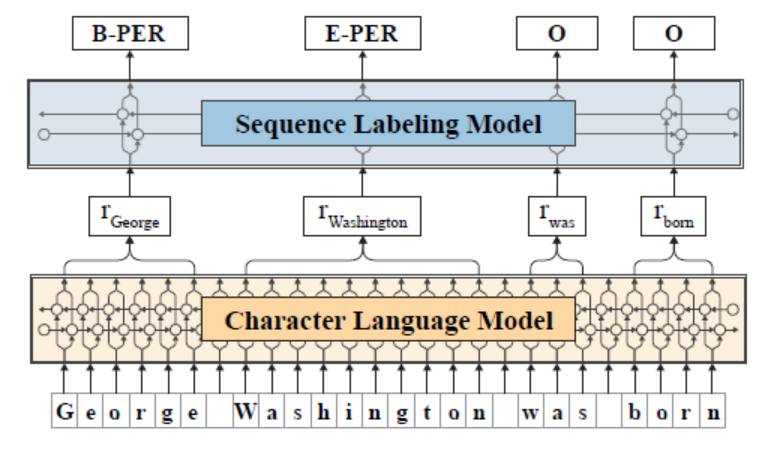
\includegraphics[scale=.5]{imagenes/2_theorical_framework/information_extraction/sequenceLabelingModel.PNG}
    \caption{Flair Sequence Labeling architecture~\cite{seqlab:flair-AkbikBBRSV19}}
    \label{fig:flairArchitecture}
\end{figure}		
	% Semantic Parsing
	\section{Semantic Parsing}
As mentioned by Kamath and Das~\cite{semPar:KamathD19}, Semantic Parsing is defined as the 
mapping from a natural language utterance into a semantic representation. These 
representations usually refer to logical forms, meaning representations or programs, which 
are executed over an underlying context such as relational tables or knowledge graphs. This 
execution yields a desired output like an answer to a question. For example, given a question 
in natural language, a semantic parser can aim to generate a valid SPARQL query based on the 
Wikidata’s ontology grammar that produces the correct answer when executed over a Wikidata 
endpoint.

The first component of a Semantic Parsing framework is the \textbf{language} to represent 
logical forms or meaning representations such as 
logic based formalisms~\cite{semPar:LiangBLFL16,semPar:ArtziFZ13}, 
graph based formalisms~\cite{semPar:BanarescuBCGGHK13,semPar:OepenKMZCFHU15} 
or programming languages~\cite{semPar:FeurerKESBH15}. In particular, we focus on query 
languages such as SQL or SPARQL. Another component is the \textbf{grammar}, which is a set of 
rules used to decide the expressivity of a semantic parser. Some examples are the Combinatory 
Categorial Grammar for complex structured queries~\cite{semPar:steedman1996}, or the Abstract 
Syntax Tree associated with a programming language’s defined grammar on general purpose code 
generation [ref]. A last component is the \textbf{underlying context}, which is the 
environment over which the output mappings are interpreted or executed. Knowledge Graphs such 
as Wikidata or DBpedia serve as examples of an underlying context.

The early attempts for Semantic Parsing were systems based on rules or statistical techniques. 
Among the rule-based systems, systems could be based on pattern matching~\cite{semPar:Johnson84a} 
or syntax-based systems~\cite{semPar:Woods73}. Though their implementation is simple, 
rule-based systems tend to be domain specific, thus hard to adapt to other domains. On the 
other hand, statistical models are able to train given examples of input-output pairs from 
any domain. Many approaches require a lexicon as a-priori 
knowledge~\cite{semPar:ZelleM96, semPar:ThompsonM03}, which is used to extract relevant 
semantic or syntactic information. Since these examples are usually manually annotated or 
require complex annotations, statistical models are hard to scale. There is also an issue 
with data sparsity, so these models only work in narrow domains.

Some of the most recent approaches that have emerged are based on Sequence-to-Sequence (Seq2seq) 
models, which usually uses an encoder-decoder framework based on neural networks. Some 
approaches implement an end-to-end paradigm where an intermediate representation is not 
needed to deliver a meaning representation; thus they do not rely on lexicons, templates or 
manually generated features. Though traditional approaches are able to better model and 
leverage the in-built knowledge of logic compositionality, approaches based on sequence 
models outperform traditional approaches due to the fact that Seq2seq-based models generalize 
better with more complex and longer sentences~\cite{semPar:JiaL16}. Furthermore, Seq2seq-based 
models can also generalize across domains~\cite{semPar:KamathD19}.

In the following subsections, we discuss in more depth how systems based on 
Sequence-to-Sequence models work. First, we will briefly explain Sequence-to-Sequence models 
along with the approach we will use in this work: the Convolutional Sequence-to-Sequence model. 
Then, we will introduce Neural Machine Translation systems and how these models can be used 
for the task of translating natural language questions to SPARQL queries.

\subsection{Sequence to Sequence models}

The Sequence-to-Sequence (Seq2seq) model was first introduced by 
Cho et al.~\cite{seqlab:ChoMBB14} [ref] for statistical Machine Translation. 
They proposed a neural network work model based on an encoder-decoder framework 
which is based on recurrent neural networks 
(RNNs)~\cite{semPar:werbos1990, semPar:rumelhart1986,seqlab:HochreiterS97}. More details 
about RNNs can be found in Appendix~\ref{appendix:neuralNetworks}.

In a Seq2seq architecture, the encoder converts a variable-length sequence into a fixed-length 
vector representation (i.e., it encodes the input sequence into a context vector) which is 
passed through to the decoder that transforms this fixed-length vector representation back 
into a variable-length sequence (i.e. decodes a context vector back to another output 
sequence). Figure~\ref{fig:seq2seqModel} illustrates graphically how a Seq2seq looks, where 
the length $T$ of the input sequence does not necessarily equal the length $T'$ of the output 
sequence.

\begin{figure}[!h]
    \centering
    
\includegraphics[scale=.5]{imagenes/insertImage.png}
    \caption{Sequence to Sequence model.}
    \label{fig:seq2seqModel}
\end{figure}

Technically, the model is learning a conditional distribution over a variable-length sequence 
conditioned on yet another variable-length sequence $p(y_1,\ldots,y_T'|x_1,\ldots,x_T)$. The 
encoder is an RNN that reads each symbol of an input sequence $x$ sequentially. While it is 
reading the current symbol on each step $t$, the hidden state $h_{<t>}^e$ of the RNN changes are
described as:

\[
    h_{<t>}^e= f(h_{<t-1>}^e,x_t)
\]

After reading the end of the sequence, the hidden state of the RNN is the summary $c$ of the 
whole input sequence, also known as its context vector. Then, the decoder is another RNN 
trained to generate the output sequence by predicting the next symbol $y_t$ given the hidden 
state $h_{<t>}^d$. This prediction is also conditioned on the previous predicted symbol 
$y_{t-1}$ and on the context vector $c$. Then, the hidden state of the decoder is defined 
for the step $t$, where $f$ is usually the \textit{sigmoid} function:

\[
    h_{<t>}^d= f(h_{<t-1>}^d,y_{t-1},c)
\]

Similarly, the conditional distribution of the next symbol, where $g$ is commonly a 
\textit{softmax} function since a valid probability must be produced, is defined as follows:

\[
    P(y_t|y_{t-1},y_{t-2},\ldots,y_1,c) = g(h_{<t-1>}^d,y_{t-1},c)
\]

Both components of the sequence model are jointly trained to maximize the following 
conditional log-likelihood function:

\[
    max_{\theta} \: \frac{1}{N} \sum_{n=1}^N log \; p(y_n|x_n)
\]

Once the model is trained, it can be used to generate a target sequence given an input 
sequence. Though Seq2seq models were originally designed based on RNNs, other variants have 
emerged~\cite{semPar:SutskeverVL14,nmt:DongL16}; among the more modern ones, a recent work 
introduces a sequence learning approach based on convolutional neural networks, which has 
shown to outperform many RNN-based models in the task of NL-to-SPARQL~\cite{nmt:nl-to-sparql-Yin19}.

\subsubsection{Convolutional Sequence to Sequence Model}
A Sequence-to-Sequence model based completely on convolutional neural networks (CNNs) is 
proposed by Gehring et al.~\cite{nmt:convS2S-GehringAGYD17}, called the Convolutional 
Sequence-to-Sequence model (ConvS2S). For this subsection we will assume a basic 
understanding of CNNs, where more details about this topic can be found on 
Appendix~\ref{appendix:neuralNetworks}.

Since CNNs do not receive the input as a sequence like RNNs do, a \textbf{position embedding} 
is proposed. First, the input elements $x=(x_1,\ldots,x_m)$ are embedded in distributional 
space as $w=(w_1,\ldots,w_m)$, where $w_j$ is a column in an embedding matrix $D$. These 
embeddings are combined with an absolute position vector $p=(p_1,\ldots, p_m)$, which 
indicates the position of the word in the sequence, in order to establish a sense of order in 
the input. From this combination the input element representation $e=(w_1+p_1,\ldots, w_m+p_m)$ 
is obtained. The output elements generated by the decoder are built using a similar 
representation.

To compute intermediate states, a simple convolutional block structure is used for both 
encoder and decoder, where such blocks are also referred to as layers. These intermediate 
states are based on a fixed number of input elements whose output for the l-th block are 
denoted as $z^l=(z_1^l,\ldots,z_m^l)$ for the encoder network and $h^l=(h_1^l,\ldots,h_m^l)$ 
for the decoder network. Each block contains a one dimensional convolution followed by a 
non-linearity.

Each convolution kernel is parameterized as $(W, b_w)$ and takes as input $X$, which is a 
concatenation of $k$ input elements embedded in $d$ dimensions, and maps them to a single 
output element $Y$. Subsequent blocks operate over the k output elements of the previous 
block. The gated linear unit (GLU)~\cite{semPar:DauphinFAG16} was chosen as the non-linearity 
to apply over the output of the convolution Y. This gating mechanism permit to control which 
input values of the current context are relevant. Aside from that, to enable deep convolutional 
networks, residual connections are added from the input of each convolution to the output of the 
block~\cite{semPar:HeZRS15}.

The input of the encoder network is padded to match the output length of the convolutional 
blocks for each block. The padding is done by adding $k - 1$ zero vectors on both the left 
and right side of the input to then remove k elements from the end of the convolution output. 
The same padding cannot be done for the decoder network since no future information is known 
beforehand~\cite{semPar:OordKK16}.

A linear mapping is added for projecting between the embedding size and the convolution 
outputs. This mapping is applied to $w$ when feeding embeddings to the encoder network, to the 
encoder output $z_j^u$, to the final block of the decoder just before the softmax $h^L$, and 
to all decoder blocks $h^l$ before computing the attention score, which is explained later. 

Lastly, a distribution is calculated over the $T$ possible next target elements $y_{i+1}$ by 
transforming the top decoder output $h_i^L$ via a linear layer with weights $W_o$ and bias 
$b_o$, as follows:

\[
    p(y_{i+1}|y_1,\ldots,y_i,x)=softmax(W_o h_i^L + b_o)
\]

Besides convolutional block structures, a separate \textbf{attention mechanism} is implemented 
for each decoder layer. Attention allows the model to focus on the relevant parts of the 
sentence for each time step. The entire process is illustrated in 
Figure~\ref{fig:convBlockStruct}. The calculation of the attention starts in the bottom left 
part of Figure~\ref{fig:convBlockStruct} with a combination between the current decoder state 
$h_i^l$ and the embedding of the previous target element $g_i$, which is defined as:

\[
    d_i^l= W_d^l h_i^l + b_d^l + g_i
\]

Then looking at the center part of Figure~\ref{fig:convBlockStruct}, for a decoder block $l$, 
the attention $a_{ij}^l$ of state $i$ and source element $j$ is computed as a dot-product 
between the decoder state summary $d_i^l$ and each output $z_j^u$ of the last encoder block $u$:

\[
    a_{ij}^l = \frac{exp(d_i^l \cdot z_j^u)}{\sum_{i=1}^m exp(d_i^l \cdot z_j^u)}
\]

Subsequently, the conditional input $c_i^l$ to the current decoder block is a weighted sum of 
the encoder outputs as well as the input element embeddings $e_j = w_j + p_j$ which corresponds 
to the center right part of Figure 1, and is defined as:

\[
    c_i^l = \sum_{j=1}^m a_{ij}^l (z_j^u + e_j)
\]

Finally, the conditional input $c_i^l$ is added to the output of the corresponding decoder layer 
$h_i^l$, as seen in the bottom right part of Figure~\ref{fig:convBlockStruct}. Compared with the 
classical single step attention, this proposal is named a multi-step attention mechanism since 
each step takes into account the attention history of the previous time steps, based on how 
conditional inputs are computed. Thus, information does not struggle to survive several steps 
as happens with recurrent networks.

\begin{figure}[!h]
    \centering
    
\includegraphics[scale=.5]{imagenes/insertImage.png}
    \caption{Convolutional block structure with a multi-step attention mechanism~\cite{nmt:convS2S-GehringAGYD17}}
    \label{fig:convBlockStruct}
\end{figure}

Some \textbf{normalization strategies} are applied to stabilize the learning process. First, 
the input and output of a residual block are summed with $\sqrt{0.5}$ to halve the variance of 
the sum. Second, the conditional input $c_i^l$ are scaled by $m\sqrt{1/m}$ to counteract any 
change in variance. Lastly, for convolutional decoders with multiple attention, the gradients 
for the encoder blocks were scaled by the number of attention mechanisms used, excluding source 
word embeddings.

Besides scaling, a \textbf{weight initialization} is also done to keep variance retained. 
Embeddings are initialized from a normal distribution with mean 0 and standard deviation 0.1. 
Weights from layers whose output is not directly fed to a GLU are initialized from 
$\mathcal{N}(0, \sqrt{1/n_l})$, where $n_l$ is the number of input connections to each neuron. 
This helps to maintain a variance of the input with a normalized distribution. Layers followed 
by a GLU are initialized from $\mathcal{N}(0, \sqrt{4/n_l})$, which is a weight initialization 
scheme based on works by He et al.~\cite{semPar:HeZRS15} and Glorot \& Bengio~\cite{semPar:GlorotB10}. 
Biases are uniformly set to zero. Lastly, dropout is applied to the input on some layers with a 
probability of p of being retained and so scaled by $1/p$, or setting them to zero 
otherwise~\cite{semPar:SutskeverVL14}.

\subsection{Natural Language to SPARQL}
Though most works have focused on translating text to SQL queries~\cite{nmt:CaiXZYLL18,nmt:ZhongCoRR17}, 
recent work has also addressed the translation of natural language to SPARQL. In particular, 
Neural Machine Translation (NMT), which involves Machine Translation systems based on Neural 
Networks, has been used to develop systems that translate questions to SPARQL queries. An 
evaluation of eight different NMT models was performed by Yin et al.~\cite{nmt:nl-to-sparql-Yin19}]. 
The NMT models included in this work were based on the aforementioned encoder-decoder Seq2seq 
architecture. Among these models, six of them are based on recurrent neural networks (RNN), 
while the remaining two are based on the ConvS2S model~\cite{nmt:convS2S-GehringAGYD17} and 
the Transformer model~\cite{semPar:VaswaniSPUJGKP17} respectively.

The systems based on RNNs include a baseline and many variants of the same LSTM architecture 
and different types of attention mechanisms. As a baseline, a Neural SPARQL Machine 
(NSpM)~\cite{nmt:nspm-SoruMMPVEN17, nmt:CoRRSoru18} is used, which consists of a 2-layer LSTM 
model with no attention mechanisms. Then, two variants of the NSpM are used with two different 
types of attention: global attention and local attention. Global attention uses the entire 
input sentence to calculate an attention vector, which complements the context vector output by 
the encoder~\cite{nlToSparql:BahdanauCB14}. On the other hand, local attention only uses a 
fixed size window around every word of the sequence to calculate a scoped attention vector per 
word~\cite{nlToSparql:LuongPM15}. Another model is based on a proposal from 
Luong et al.~\cite{nlToSparql:LuongPM15}, which consists of a 4-layers LSTM model with local 
attention. Lastly, the Google Machine Translation (GNMT) architecture~\cite{nlToSparql:WuSCLNMKCGMKSJL16} 
is included with two different variants: a 4-layer LSTM and a 8-layer LSTM, both with local 
attention. The only difference between Luong’s model and the GNMT is that the second model 
includes residual connections from the third layer and uses a bidirectional LSTM in the first 
layer of the encoder.

\subsubsection{Neural Machine Translation}

Though the architecture of each model varies, the encoding of SPARQL queries used in all 
approaches is the same as that proposed by Soru et al.~\cite{nmt:nspm-SoruMMPVEN17}. Their 
encoding suggests that URIs are abbreviated using their prefixes  followed by an underscore; 
brackets and dots are replaced by their verbal description, and SPARQL keywords are lower-cased. 
For example, a query over Wikidata is shown in Listing~\ref{lst:decodedWikidataSparqlExample}, 
when after an encoding conversion, it is converted to an encoded query as seen in 
Listing~\ref{lst:encodedWikidataSparqlExample}.

\begin{lstlisting}[captionpos=b, 
    caption=SPARQL query before encoding., 
    label=lst:decodedWikidataSparqlExample,
    basicstyle=\ttfamily,frame=single]
PREFIX wd: <http://wikidata.org/wiki/>
PREFIX wdt: <http://wikidata.org/prop/direct/>

SELECT ?sbj 
WHERE {
    ?sbj wdt:P19 wd:Q201007 .
    ?sbj wdt:P166 wd:Q37922 .
}
\end{lstlisting}

After training, the system will output an encoded form that can be transformed back to the 
original SPARQL representation. 

\begin{lstlisting}[captionpos=b, 
    caption=SPARQL query after encoding (note it excludes the PREFIX clauses)., 
    label=lst:encodedWikidataSparqlExample,
    basicstyle=\ttfamily,frame=single]
select var_sbj where brack_open var_sbj wdt_p19 
wd_q201007 sep_dot var_sbj wdt_p166 wd_q37922 
sep_dot brack_close
\end{lstlisting}

The evaluation metrics typically used to compare these systems are string-matching accuracy, 
BLEU score and perplexity. The string-matching accuracy is used to measure the amount of exact 
matches delivered by each system. The global accuracy is then the percentage of cases that are 
syntactically equal to the expected answer. This metric is particularly useful when measured 
over a dataset based on SPARQL templates, giving insights into whether or not the expected 
SPARQL form is being correctly generated.

The Bilingual Evaluation Understudy (BLEU) score is used to measure how similar two sentences 
are by using a geometric average of modified n-gram precision~\cite{nlToSparql:PapineniRWZ02}, 
which is represented by the following formula:

\[
    BLEU = BP \cdot exp(\sum_{n=1}^N w_n \; log \: p_n)    
\]

The modified precision $p_n$ for each candidate counts the number of times an n-gram occurs in a 
reference translation(s), takes the maximum count of each n-gram among the reference(s), and 
then clips the count of each n-gram in the candidate translation to the maximum count. To avoid 
short candidate translations getting higher scores than desired, a brevity penalty (BP) is 
applied which is set to 1 if the candidate length $c$ is larger than the maximal reference 
length $r$ or set to $exp(1-r/c)$ otherwise. The wn represents weights for each modified 
precision. By default $w_n=\frac{1}{N}$ and $N=4$. In this case, the BLEU score goes from 0 to 
100, where a score closer to 100 means the model is performing better. Note that BLEU does not 
account for word order. 

\textbf{Perplexity} is used to understand the model’s intrinsic behavior based on a cross 
entropy H(p,q) which is defined as follows:

\[
    H(p,q)= -\sum_x p(x) \; log \: q(x)
\]

where $p$ represents the target probability distribution and q is the estimated probability 
distribution. Their similarity is defined by all possible values $x$ in the distribution. In 
this case, $p$ is the one-hot encoding vector of the target vocabulary and q is deduced from 
the result of the output softmax layer. Then the perplexity is defined as the exponentiation 
of the cross entropy:
\[
    perplexity(p,q)=2^{H(p,q)}
\]

According to the experiments conducted by Ying et al.~\cite{nmt:nl-to-sparql-Yin19}, the model 
that performs best was the ConvS2S model. Although many datasets were used in their experiments, 
we are only interested in LC-QuAD~\cite{dataset:lcquad2-DubeyBA019} and 
DBNQA~\cite{dataset:dbnqa-hartmann-marx-soru-2018}, two datasets that represent opposite traits 
of a Question Answering Dataset: the LC-QuAD dataset contains few questions (5000) but with high 
complexity and high variance of its questions while the DBNQA dataset contains a huge volume of 
questions (nearly 900,000) but it lacks variety in its questions. We explain with more details 
what we understand by a “good dataset” in the \textit{Question Answering} section. The results 
of the three best models among the eight selected over the mentioned datasets are shown in 
Table~\ref{table:nmtYinResults}.

\begin{table}[h!]
    \centering
    \resizebox{\textwidth}{!}{%
    \begin{tabular}{|l|l|l|l|l|l|l|l|l|l|l|l|l|}
    \hline
    \multirow{2}{*}{} & \multicolumn{4}{c|}{Perplexity}                           & \multicolumn{4}{c|}{BLEU Score}                           & \multicolumn{4}{c|}{Accuracy}                             \\ \cline{2-13} 
                    & \multicolumn{2}{c|}{LC-QuAD} & \multicolumn{2}{c|}{DBNQA} & \multicolumn{2}{c|}{LC-QuAD} & \multicolumn{2}{c|}{DBNQA} & \multicolumn{2}{c|}{LC-QuAD} & \multicolumn{2}{c|}{DBNQA} \\ \hline
    Models            & Train         & Valid        & Train        & Valid       & Valid         & Test         & Valid        & Test        & Valid         & Test         & Valid        & Test        \\ \hline
    LSTM\_Luong       & 1.12          & 4.92         & 1.9          & 2.15        & 52.43         & 51.06        & 77.64        & 77.67       & 0             & 0            & 34           & 34          \\ \hline
    ConvS2S           & 1.14          & 3.25         & 1.12         & 1.25        & 61.89         & 59.54        & 96.05        & 96.07       & 8             & 8            & 85           & 85          \\ \hline
    Transformer       & 1.16          & 3.15         & 2.21         & 3.34        & 58.99         & 57.43        & 68.68        & 68.82       & 7             & 4            & 3            & 3           \\ \hline
    \end{tabular}%
    }
    \caption{Performance comparison of three models included in Yin et al.\cite{nmt:nl-to-sparql-Yin19}}
    \label{table:nmtYinResults}
\end{table}

Based on the perplexity results, there is a serious overfit for all models over the LC-QuAD 
dataset which Yin et al. attributes to the small size of the dataset and its complex questions. 
No evident overfit is spotted over DBNQA, and the ConvS2S shows better results which is 
reflected in the other results as well. The BLEU score results reflect that ConS2S again 
outperformed all other models and shows a correlation between perplexity and BLEU, especially 
when looking at DBQNA results. Finally, accuracy results clearly show that RNN based models and 
the Transformer do not perform positively in any case when compared to the ConvS2S model. 
However, the results over the LC-QuAD again shows there is still a challenge to handle more 
complex questions among all NMT models.

	
	% Question Answering over Knowledge Graphs
	\section{Question Answering over Knowledge Graphs}
\label{cap2:qakg}
Question Answering systems respond to the need to access information on the Web without 
detailed knowledge of Semantic Web technologies such as how data is structured (RDF) or how to 
access data (SPARQL). In particular, Question Answering systems (QAS) provide end-users with an 
intuitive and easy-to-use user interface, which hides the complexity behind the Semantic Web 
standards~\cite{qa:intro-UngerFC14}. These systems differ from traditional search engines such 
as Google in that search engines only return documents in which the answer can be potentially 
found, whereas a Question Answering system aims to return precise answers~\cite{qa:LopezUSM11}.

When we mention the task of Question Answering over Knowledge Graphs (QAKG), we refer to 
receiving a natural language question and returning an answer retrieved from one or more 
Knowledge Graphs (e.g. the first man to walk on the moon is Neil 
Amstrong\footnote{\url{https://www.wikidata.org/wiki/Q1615} in Wikidata}). Though there is work which 
includes a wider context along with the question, such as hybrid questions or chain of questions, 
we focus only on the problem of responding to an individual question without further context 
besides the question itself.

Another consideration for defining the scope of Question Answering is the question and answer 
type a system aims to respond to/with. Among the types of questions for which a Question 
Answering system usually provides an answer are:

\begin{itemize}
    \item \textbf{Definition question}, refers to a definition of a subject or object (e.g. 
    \textit{“Who was Violeta Parra?”}).
    \item \textbf{Factoid questions}, which are related to facts. This type of questions 
    includes three different variants:
    \begin{itemize}
        \item \textbf{Predicative questions} that refer to a specific object related to a predicate 
        such as who, what, where, how (e.g. \textit{“Who was the first man in space?”}, 
        \textit{“What is the highest mountain in Chile?”}).
        \item \textbf{List questions} that refer to all the answers that fulfill the fact being 
        asked (e.g. \textit{“Give me all the countries in America“}).
        \item \textbf{Boolean questions} that refer to whether the fact being questioned is true 
        or not (e.g. \textit{“Was Gabriela Mistral a poet?”}).
    \end{itemize}
\end{itemize}

In the context of Linked Data, a Question Answering system is limited to the information the 
available knowledge graphs can represent. For instance, questions not based on specific facts 
such as process questions (e.g. \textit{“How do I make a lemon pie?”}) or opinion questions 
(e.g. \textit{“What do most Chileans think of global warming?”}) cannot be answered.

Questions can also be classified depending on the answer type expected. One example is the work 
of Xin Li et al.~\cite{qa:LiR02}, which classify questions given five high-level categories: 
\textbf{entities} (e.g. event, color, animal, plant), \textbf{descriptions} (e.g. definition, 
manner, reason), \textbf{humans} (e.g. individual, group), locations (e.g. city, country, 
mountain) and numbers (e.g. count, date, distance, size). Another way is to classify questions 
according to its \textbf{focus} and \textbf{topic}, representing what the question is about. 
For instance, the question \textit{“What is the height of Aconcagua mountain?”} focuses on the 
property height in the topic of geography while the question \textit{“What is the best 
height-increasing drug?”} focuses on the same property, but a different topic, which is medicine.

According to Fu et al.~\cite{qa:FuQTLYS20abs-2007-13069}, current systems do not struggle with 
answering simple questions, i.e. questions that only require one subject-predicate-object 
triple fact, but complex questions are still a challenge for QAKG. A complex question usually 
is referred to as three types: questions under specific conditions (e.g. \textit{“Who was the 
president of Chile during the Great Recession of 2008?”}), questions with more intentions (e.g. 
\textit{“Give the names of the Chilean national football team and the number of goals they have 
scored”}), and questions requiring constraint inference (e.g. \textit{“What is the most 
expensive movie starring Pedro Pascal?”}).

\subsection{QAKG approaches}
\label{cap2:qakg/approaches}
Though there is no standard approach for QAKG, most techniques or methods proposed follow a 
similar four-stage pipeline~\cite{qa:core-techniques-DiefenbachLSM18}. First, a question 
analysis stage includes techniques that extract information from the current question using 
purely syntactic features. Then, the phrase mapping stage defines techniques that identify KG 
resources for each named entity and its dependencies. Next, the disambiguation stage 
encapsulates techniques that rank and determine for each named entity the most relevant 
resources according to the context of the question. Lastly, the query construction stage 
considers techniques used to construct the SPARQL query that should retrieve the final answer. 
In summary, most Question Answering systems are a combination of these four steps and vary with 
respect to which techniques are used to address each phase of the Question Answering process.

On the other hand, QAKG approaches can be classified according to which techniques their models 
are based on. The traditional QAKG models rely on predefined templates and manuals to parse 
questions [ref]. However, these traditional approaches require a certain level of knowledge of 
linguistics, and tend to be difficult to scale. Therefore, recent work has focused more on two 
kinds of approaches: methods based on Information Retrieval methods and other ones based on 
Neural Semantic Parsing.

\subsubsection{Information Retrieval-based methods}
\label{cap2:qakg/approaches/infRetrieval}
Information Retrieval (IR) based models reduce the QA task to binary classification or sorting 
over candidate answers. An IR-based method usually begins by identifying relevant entities 
mentioned in the question. Then, it extracts topic-entity-centric subgraphs where all nodes are 
considered candidate answers. Next, candidates are scored using features that provide semantic 
relevance and help to select the final answers. Depending on how the feature representations 
are built, IR-based methods can be divided into those based on feature engineering and those 
based on representation learning.

Methods based on feature engineering rely on manually defined and extracted features. For 
example, Yao et al.~\cite{qa:YaoD14} extract four types of features based on the question’s 
syntactic information, which includes question words, question focus words, topic words, and 
central verbs. These features are used in a classification model to determine the final answer. 
However, building these features is time-consuming and is not able to capture the entire 
semantic information of questions.

Methods based on representation learning convert questions and candidate answers into vector 
representations and reduce QAKG to a semantic matching computation between representations of 
questions and their candidate answers. Some methods incorporate external knowledge to complement 
the representation information and address the incompleteness that the KG might 
have~\cite{qa:XuRFHZ16,qa:SunDZMSC18,qa:TrouillonWRGB16}. Some other methods incorporate a 
multi-hop reasoning process to handle more complex questions~\cite{qa:SukhbaatarSWF15,qa:MillerFDKBW16,qa:QiuWJZ20}.

Overall, IR-based models get rid of manually defined templates and rules, and can follow an 
end-to-end training. However, these methods lack model interpretability and are not able to 
handle complex questions that require constraint inference.

\subsubsection{Neural Semantic Parsing-based methods}
\label{cap2:qakg/approaches/neuSemParsing}
In this context, methods based on Semantic Parsing aims to convert natural languages into 
executable query languages. Methods based on Neural Semantic Parsing (NSP) rely on Neural 
Networks to enhance the parsing capacity and scalability, instead of relying on predefined 
templates or rules. Thus, these models aim to map unstructured questions to intermediate 
logical forms which are later converted to structured queries.

One approach is to use query graphs, which are graphs that encoded questions, have strong 
representation ability and share topological commonalities with knowledge graphs. One example 
is GraphParser, proposed by Reddy et al.~\cite{qa:ReddyLS14} which frames the Semantic Parsing 
problem as a Graph Matching problem. Derived from GraphParser, the Staged Query Graph 
Generation~\cite{qa:YihCHG15} (STAGG) and the Multiple Constraint Query Graph~\cite{qa:BaoDYZZ16} 
(MultiCG) were proposed. While STAGG proposed a different construction of the query graph based 
on a restricted subset of lambda-calculus in the graph representation, MultiCG extends STAGG to 
include more constraint types and operators in order to cover more complex questions. Since all 
these proposals rely on Entity Linking tools to initialize the query graph construction, 
Yu et al.~\cite{qa:YuYHSXZ17} assumes a poor performance of such tools and proposes a 
Hierarchical Residual BiLSTM with the goal of improving entity recognition accuracy.

On the other hand, other work proposes to use encoder-decoder models to reduce the Semantic 
Parsing task into a Sequence-to-Sequence problem. One example is the Seq-to-Tree model proposed 
by Dong et al.~\cite{nmt:DongL16} that uses a hierarchical tree-structured decoder to capture 
the structure of logical forms. Then, in order to take more advantage of the syntactic 
information of the input question, the Graph-to-Seq model was proposed by Xu et al.~\cite{qa:XuWWYCS18} 
to encode the question as a syntactic graph. A last example is the Neural Symbolic Machine 
proposed by Liang et al.~\cite{qa:LiangBLFL17}, which proposed a lighter supervision approach 
by training a Seq-to-Seq model with reinforcement learning. Nevertheless, none of the examples 
mentioned above have been evaluated in the context of QAKG.

In general, the results of NSP-based models tend to be slightly better than the results from 
IR-based models. Nevertheless, it is still challenging to train a Neural Semantic Parser due to 
the lack of training data.

\subsection{Main Challenges}
\label{cap2:qakg/challenges}
The QAKG task is still an open problem, where many challenges have partially been addressed. 
Some of these challenges are related to the question being asked and others to the answers that 
can be returned. 

There are different ways to express the same question, as there are different ways to represent 
information within Knowledge Graphs. The \textbf{lexical} gap is the difference between the 
vocabulary used in a question and how information is expressed in the Knowledge 
Graph~\cite{semPar:lexical-gap-HakimovUWC15}. The bigger this gap is, the more difficult it is 
for QA systems to locate the correct resources for each named entity identified. 

Some work has tried to address the lexical gap, where most techniques are based on string 
normalization, pattern matching or entailment. For example, string normalization methods such 
as converting to lower case or stemming (e.g. convert \textit{“writing”} to its base form 
\textit{“write”}) help to reduce the search space when mapping entities. Another example are 
pattern libraries, such as PATTY~\cite{qa:NakasholeWS12} or BOA~\cite{qa:GerberN12}, that 
support pattern matching from a phrase to a resource. Nevertheless, most techniques proposed 
are based on manually defined rules, which is hard to scale or to transfer to other Knowledge 
Graphs.

Another challenge related with input expressivity is the \textbf{ambiguity} bound to each 
question, in other words, questions with different semantic meaning but with similar syntactic 
structure. There two main types of ambiguities: homonymy, when different concepts are 
represented by a string with the same spelling (e.g. the word \textit{“right”} can refer to 
\textit{“correct”} or \textit{“direction opposite to left”}), and polysemy, when one string can 
represent different but related concepts (e.g. \textit{“newspaper"} can refer to a 
\textit{”printed publication”} or to a \textit{”media company”}). 

Among the approaches used to address ambiguity are corpus-based methods or resource-based 
methods. Usually the corpus-based methods use statistical models from unstructured text 
corpora~\cite{qa:shirai1997,qa:ShenYYJLC11}. On the other hand, resource-based methods take 
advantage of the RDF properties of candidate resources. A score is calculated for each entity 
following the assumption that a better score applies a higher probability of a resource to be 
chosen. Some examples are RVT, which uses Hidden Markov Models~\cite{qa:GiannoneBB13}; CASIA, 
which relies on Markov Logic Networks~\cite{qa:shizhu2014casia}; or Treo~\cite{qa:freitas2011treo,
qa:FreitasOOSC13}, which uses Wikipedia-based semantic relatedness.

Unlike the lexical gap, which affects the recall of a QA system, ambiguity negatively affects 
its precision. While some methods aim to reduce the lexical gap, these same methods can make it 
difficult to address ambiguity. It is customary that in the disambiguation stage the systems 
try to balance the effects of both issues.

From challenges that are related to the query construction, the needs of \textbf{complex operators} 
affect the capability of a QA system to respond to more complex questions. The difficulty to 
handle a question increases when several facts have to be identified. Some examples that have 
tried to addresses these issue are YAGO-QA~\cite{qa:AdolphsTSUW11}, which tries to address 
nested questions; PYTHIA~\cite{qa:UngerC11}, which can answer question involving quantifiers, 
comparatives, superlatives and others; and IBM Watson~\cite{qa:GliozzoK12}, which can respond 
to indirect questions and multiple sentences.

As mentioned before, there are certain types of questions that current QA systems struggle to 
handle. One example is that of \textbf{procedural questions} (i.e. describe a procedure), which 
no QA system has been able to solve. Another example relates to \textbf{temporal questions} 
which refer to questions that require inferring temporal relation between events, though some 
works have tried to address temporal questions~\cite{qa:Allen83,qa:FerrandezSKDFNITONMG11,
qa:MeloRN11}. A last example relates to \textbf{spatial questions} that include questions 
referring to locations. The capability of answering spatial questions depends on how the schema 
of the knowledge represents locations (e.g. latitude and longitude), and how QA systems can use 
that information to enrich semantic data~\cite{qa:YounisJTA12,qa:graph-2-ZouHWYHZ14}.

The use of \textbf{templates} is thus more common to construct SPARQL queries that include 
complex operators such as aggregation or filter functions. These SPARQL query templates can be 
either manually or automatically created. One template-driven approach is Casia~\cite{qa:shizhu2014casia} 
that uses the question type, named entities and POS tagging techniques to generate graph 
pattern templates from which a SPARQL query is built. Other approaches use manually created 
templates combined with machine learning methods~\cite{qa:AbachaZ12}. 

\subsection{Benchmark \& Datasets}
\label{cap2:qakg/benchmarkDatasets}
In order to measure a Question Answering system performance, the most common parameters used 
across all benchmarks are \textbf{Precision}, \textbf{Recall} and \textbf{F1-score}. These 
three metrics usually are based on a gold standard set per question, which are the entities or 
values expected to be returned by the QA system. Given a question $q$, the formulas for Recall, 
Precision and F1-score are represented in the following formulas:

\begin{equation}
    \begin{aligned}
    Recall(q) &= \frac{\mbox{number of correct system answers for q}}{\mbox{number of gold standard answers for q}} \\
    Precision(q) &= \frac{\mbox{number of correct system answers for q}}{\mbox{number of system answers for q}} \\
    F1(q) &= \frac{2 \ast Precision(q) \cdot Recall(q)}{Precision(q)+Recall(q)}
    \end{aligned}
\end{equation}

As an example, given the question \textit{“Which are the primary colors?”}, the gold standard 
answer would be [\textit{“red”}, \textit{“green”}, \textit{“blue”}]. If a system answer is [
\textit{“brown”}, \textit{“green”}], the Precision would be 0.5 since \textit{“green”} is the 
only color part of the correct answers among the two colors returned, while the Recall would be 
0.33 because the only color correctly returned among the golden standard set is \textit{“green”}.

Similar to Entity Linking system evaluations, the global precision or global recall can be 
reported in two ways: as a micro average or a macro average. The F1-score is also used to 
combine  precision and recall into one measure.

In recent years, many datasets have been developed to include complex questions. In particular, 
we will briefly describe the datasets used in this work whose questions often require complex 
query construction and provide the expected query and result.

\subsubsection{QALD}
\label{cap2:qakg/benchmarkDatasets/qald}
The series of QALD datasets are part of the Question Answering over Linked Data (QALD) challenges, 
which aim to provide an up-to-date benchmark for measuring performance and comparing Question 
Answering systems~\cite{qa:qald-Lopezetal2013}. The QALD challenge is divided into multiple 
tasks that invite QA systems to address different challenges of Question Answering: 
multilinguality, hybrid questions, large-scale question answering and adaptability to other 
data sources. Though most versions of QALD contain questions that can be only answered over 
DBpedia, one of the versions of QALD did contain questions over Wikidata for the task of 
adaptability.

That being said, the $7^{th}$ version of QALD (QALD-7)~\cite{dataset:qald7-UsbeckNHKRN17} includes a 
dataset of 150 questions over Wikidata, divided into 100 questions for training and 50 for 
testing. The questions comes from a real-world question and query logs, where each question is 
manually annotated and includes a manually specified SPARQL query. Regarding the complexity of 
the questions, about 38\% are considered complex, including questions with counts, superlatives, 
comparatives, and temporal aggregations.

Despite the good quality of the questions of QALD-7 and its proximity to real-world questions, 
its limited size means that it is insufficient for training NSP-based models, which require a 
considerable amount of annotations to undergo a successful learning process

\subsubsection{LC-QuAD}
\label{cap2:qakg/benchmarkDatasets/lcquad}
The Large-Scale Complex Question Answering Dataset (LC-QuAD) is a dataset based on 
DBpedia~\cite{dataset:lcquad-TrivediMDL17}, where 82\% of its questions are considered complex. 
Differently from QALD, the SPARQL queries are built using a relatively small number of 
predefined templates, thus generating a large high-quality dataset with low domain-expert 
intervention. This results in a dataset that contains a total of 5000 questions with their 
corresponding queries.

Their dataset construction pipeline follows a different proposal to the standard one, where 
instead of writing the natural language question and then its logical form (aka the SPARQL 
query), the process is inverted. Thus the process starts by filling 38 hand-made SPARQL 
templates with seed entities and relations from a preferred predicate list to generate specific 
SPARQL queries. After that, a natural language question (NLQ) is deduced, for each generated 
SPARQL query, following a three-step process: a generation of a normalized NLQ by filling a 
Normalized Natural Question Template (NNQT) with the entity and relations names used to 
generate the current query, a verbalisation of the normalized NLQ using crowdsourcing tools, 
and a final validation done by an independent reviewer.

The proposal of LC-QuAD was a first step to allow NSP-based models to be applied to the field 
of Question Answering in the RDF/SPARQL setting, though most works~\cite{qa:FuQTLYS20abs-2007-13069} 
show that a larger amount of examples are still required to train models properly.

\subsubsection{DBNQA}
\label{cap2:qakg/benchmarkDatasets/dbnqa}
The DBpedia Neural Question Answering (DBNQA) [ref] dataset is thus far the largest dataset for 
Neural Question Answering over DBpedia, with 894,499 annotated pairs. The process to construct 
this dataset is similar to the one proposed for LC-QuAD, though its templates are extracted 
from the multilingual QALD-7 train dataset that includes 215 questions (not the same dataset as 
the Wikidata QALD-7 dataset mentioned before) and the same LC-QuAD dataset. This extraction 
process provides 5217 SPARQL templates. Another difference is the approach to generate natural 
language questions. This dataset originated from the purposes of training Neural SPARQL 
Machines, mentioned in the \textit{Semantic Parsing} section.

The template extraction process for each case consisted of replacing the concrete entities 
with placeholders. This is the case for the original question, where resource labels are 
replaced, and the query, where entities are replaced. This process functioned differently for 
the two datasets used. For the QALD-7-Train~\cite{dataset:qald7-UsbeckNHKRN17} dataset the 
resources were manually replaced, while for LC-QuAD an automatic script was implemented taking 
advantage of the fact that the resources were marked in the questions. As an example, given the 
question \textit{“What are the artists that are born in Stockholm?”} which generates the query 
in Listing~\ref{lst:dbnqaSparqlExample}, the template extraction process would return a 
question template \textit{“What are the artists that were born in <A>?”}, replacing the 
resource Stockholm, and would generate the query template shown in Listing~\ref{lst:dbnqaTemplateExample}.

\begin{lstlisting}[captionpos=b, 
    caption=SPARQL query for the question: \textit{"What are the artists that are born in Stockholm?"}., 
    label=lst:dbnqaSparqlExample,
    basicstyle=\ttfamily,frame=single]
SELECT DISTINCT ?sbj WHERE {
    ?sbj dbp:placeOfBirth dbr:Stockholm .
    ?sbj rdf:type dbo:MusicalArtist .
}
\end{lstlisting}

\begin{lstlisting}[captionpos=b, 
    caption=Query template for the question: \textit{"What are the artists that are born in <A>?"}., 
    label=lst:dbnqaTemplateExample,
    basicstyle=\ttfamily,frame=single]
SELECT DISTINCT ?sbj WHERE {
    ?sbj dbp:placeOfBirth <A> .
    ?sbj rdf:type dbo:MusicalArtist .
}
\end{lstlisting}

Then, the dataset is constructed following a similar approach to the one used for LC-QuAD. 
First, a set of entities is chosen per query template, where the entities selected are the ones 
that contain the relations contained in the query (e.g. if the property location is contained 
in the query, places would be selected accordingly). Then the selected entities are used to 
generate each SPARQL query with its corresponding NLQ. 

Since the construction of each case does not include a paraphrasing stage, there is almost no 
variation of questions that comes from the same template, i.e. there was no syntactic 
difference for questions with the same purpose. This lack of variation negatively affects the 
generalisation capabilities of NSP-based models trained on this dataset~\cite{qa:BerantL14}.

\subsubsection{LC-QuAD-2}
\label{cap2:qakg/benchmarkDatasets/lcquad2}
Taking into account all the advantages and disadvantages of the aforementioned datasets, a 
second version of the Large-Scale Complex Question Answering Dataset (LC-QuAD-2) was 
proposed~\cite{dataset:lcquad2-DubeyBA019}. In particular, this dataset provides around 30,000 
questions over Wikidata which contains complex questions and high diversity among its questions. 
The dataset generation workflow combines semi-automatic question generation along with a 
crowdsourced-based paraphrasing phase.

SPARQL queries are generated given a set of entities, predicates and templates) do not differ 
much compared to the first version of LC-QuAD. Nevertheless, the SPARQL templates used are 
different from the ones used before. Now the templates are based on one of the 10 types of 
question LC-QuAD-2 aims to address:

\begin{enumerate}
    \item \textbf{Single fact}: use a single (S-P-O) triple query, e.g. \textit{"Who is the 
    screenwriter of Mr. Bean?"}.
    \item \textbf{Single fact with type}: the fact is focused on the type of constraint, e.g. 
    \textit{"Billie Jean was on the tracklist of which studio album?"}.
    \item \textbf{Muti-fact}: use two connected facts, e.g. \textit{"What is the name of the 
    sister city tied to Kansas City, which is located in the county of Seville Province?"}.
    \item \textbf{Fact with qualifiers}: includes more informative facts stored in qualifier 
    properties, e.g. \textit{"What is the venue of Barack Obama’s marriage ?"}.
    \item \textbf{Two intentions}: consider questions with two intentions and also rely on 
    qualifiers, e.g. \textit{"When and where did Barack Obama get married to Michelle Obama?"}.
    \item \textbf{Boolean}: ask whether a fact is true or false, including questions with 
    number as an object, e.g. \textit{"Did Breaking Bad have 5 seasons?"}.
    \item \textbf{Count}: uses the COUNT keyword to perform a numeric count over a certain fact, 
    e.g. \textit{"What is the number of Siblings of Edward III of England ?"}.
    \item \textbf{Ranking}: requires counting and sorting in order to rank entities regarding a 
    certain property, e.g. \textit{"What is the binary star which has the highest color index?"}.
    \item \textbf{String Operation}: applies string operations at a work or character level, 
    e.g. \textit{"Give me all the Rock bands that start with the letter R?"}.
    \item \textbf{Temporal aspect}: covers temporal properties where various time facts are 
    included in qualifier properties, e.g. \textit{"With whom did Barack Obama get married in 1992?"}.
\end{enumerate}

Considering that some types of questions might have more than one SPARQL template variation, a 
total of 22 templates are used. 

\begin{figure}[!h]
    \centering
    
\includegraphics[scale=.45]{imagenes/insertImage.png}
    \caption{Example of LC-QuAD 2 question workflow generation.}
    \label{fig:lcquad2Pipeline}
\end{figure}

Then, a set of relevant entities and a predicate list is selected based on each SPARQL template, 
meaning that each question type includes different entities and properties (e.g. the property 
\textit{“birthPlace”} might not be used for questions that require counting). For each case, a 
subgraph is built based on three factors: an entity, the SPARQL template, and one or more 
suitable predicates. From each subgraph a SPARQL query is generated. Next, each SPARQL query is 
transformed to a normalized natural language question, called a Question Template (QT), which is 
then verbalised and paraphrased in a three-step pipeline based on human turkers from the Amazon 
Mechanical Turk tool (a crowdsourcing tool to perform simple tasks on a large scale). 

The first step is to convert each QT into Verbalised Question (QV), where most of the 
grammatical errors and semantic inconsistencies of the QT are fixed. The second step is to 
paraphrase each QV, where the resulting Paraphrased Question (QP) should preserve the overall 
semantic meaning while changing its syntactic content and structure. An example of the entire 
generation of one case is illustrated in Figure~\ref{fig:lcquad2Pipeline}. The last step is a 
human verification where a comparison is done between each QT with its corresponding QP in 
order to measure the quality of the final result in terms of semantic similarity.

After the entire generation process, a dataset is provided with around 52\% complex questions 
and significant variation in their  question structure. There is, however, a small percentage 
of error derived from using a crowdsourcing tool [ref], with questions losing part of their 
semantic intent or questions that are poorly verbalized/paraphrased, which should be taken into 
consideration when using this dataset to train NSP-based models. 
	
% Trabajo relacionado
% Baseline
% Sistema propuesto
%\chapter{Segundo}
\lipsum[1-3]
    \lipsum[30-35]
	\begin{enumerate}
		\item Item 1
		\begin{enumerate}
			\item Subitem 1
			\item Subitem 2 (ver Figura \ref{logofcfm})
		\end{enumerate}
		\item Item 2
		\item Item 3
	\end{enumerate}
	\begin{teo}
	Se tiene que $$\int_0^t e^sds=e^t-1.$$
	\end{teo}
	\lipsum[36-40]
\begin{defn}[ver \cite{rdf}] Definición definitiva $$\frac{d}{dx}\int_a^xf(y)dy=f(x).$$\end{defn}
\lipsum[50-60]
%\input{conclu.tex}

% \input{glosario.tex} % opcional

\bibliographystyle{plain}
\bibliography{bibliografia}

% \input{anexo_apendices.tex} % opcionales

\end{document}
